


\newcommand\scaleSLIBIMER{0.175}

SLIs are obtained by applying the discretization process described in $\S$\ref{subsec:SLI_spatial_discretization} to the previously shown sprays. Since it was shown in the former section that convergence was achieved for most magnitudes at $x_c = 2$ mm, SLIs are shown here only for the sampling planes at $x_c = 1.5, 2$ mm. Results are shown in Figures \ref{fig:injectors_sli_BIMER_DX10_xD05} to  \ref{fig:injectors_sli_BIMER_DX15_xD06p67}. The SMDs maps show a circular structure in which large values are obtained at the center of the spray and diameters are reduced further away. Fluxes maps exhibit a circular structure which is typical from all liquids JICF. These maps show maximum flux values located at around $y_c = 0$ and symmetry with respect to this axis for case DX10, which indicates that the crossflow direction has been properly chosen. Axial velocity maps show a classical a low-velocity region in the bottom part, central region of the spray which corresponds to the disturbance effect of the spray, while the vertical velocity maps display the classical layered structure with increasing velocity along the vertical direction $z_c$, hence indicating that the spray continues to penetrate further away as it is convected downstream. Large differences with respect to the classical JICF of Chapter \ref{ch5:jicf_resolved_simulations} are observed for the lateral velocity $v_c$, since in this case the profiles are not symmetric with respect to the $y_c = 0$ axis due to the swirl component of the air. With respect to the convergence maps, it is shown that more converged probes are obtained for the fine resolution than for the coarse one even though the total physical time simulated is lower. The same observation was done for the classical JICF as detailed in $\S$\ref{sec:ch5_learning_SLI}: it can be concluded then that a finer mesh makes SLI converge with lower physical time simulated. It is worth to note that the convergence has only been defined according to the droplet size distribution as indicated by Eq. (\ref{eq:MSE_definition}): further research includes testing other $MSE$ functions accounting for other magnitudes such as velocities. Nevertheless, the $SMD$ and velocity maps obtained for the coarse resolution (Figures \ref{fig:injectors_sli_BIMER_DX15_xD05} and \ref{fig:injectors_sli_BIMER_DX15_xD06p67}) seem \textsl{less converged} than their equivalents for the fine case (Figures \ref{fig:injectors_sli_BIMER_DX10_xD05} and \ref{fig:injectors_sli_BIMER_DX10_xD06p67}) due to the less smooth contours obtained. This might indicate that the resolution DX15 is too coarse to simulate BIMER, and therefore only the SLI obtained for case DX10 will be used to perform the dispersed phase simulations from Chapter \ref{ch9:BIMER_lagrangian}.


\subsubsection*{Case DX10}



%%%%%%%%%%%%%%%% DX10, xD = 5


\begin{figure}[h!]
\centering
\begin{subfigure}[b]{0.3\textwidth}
	\centering
   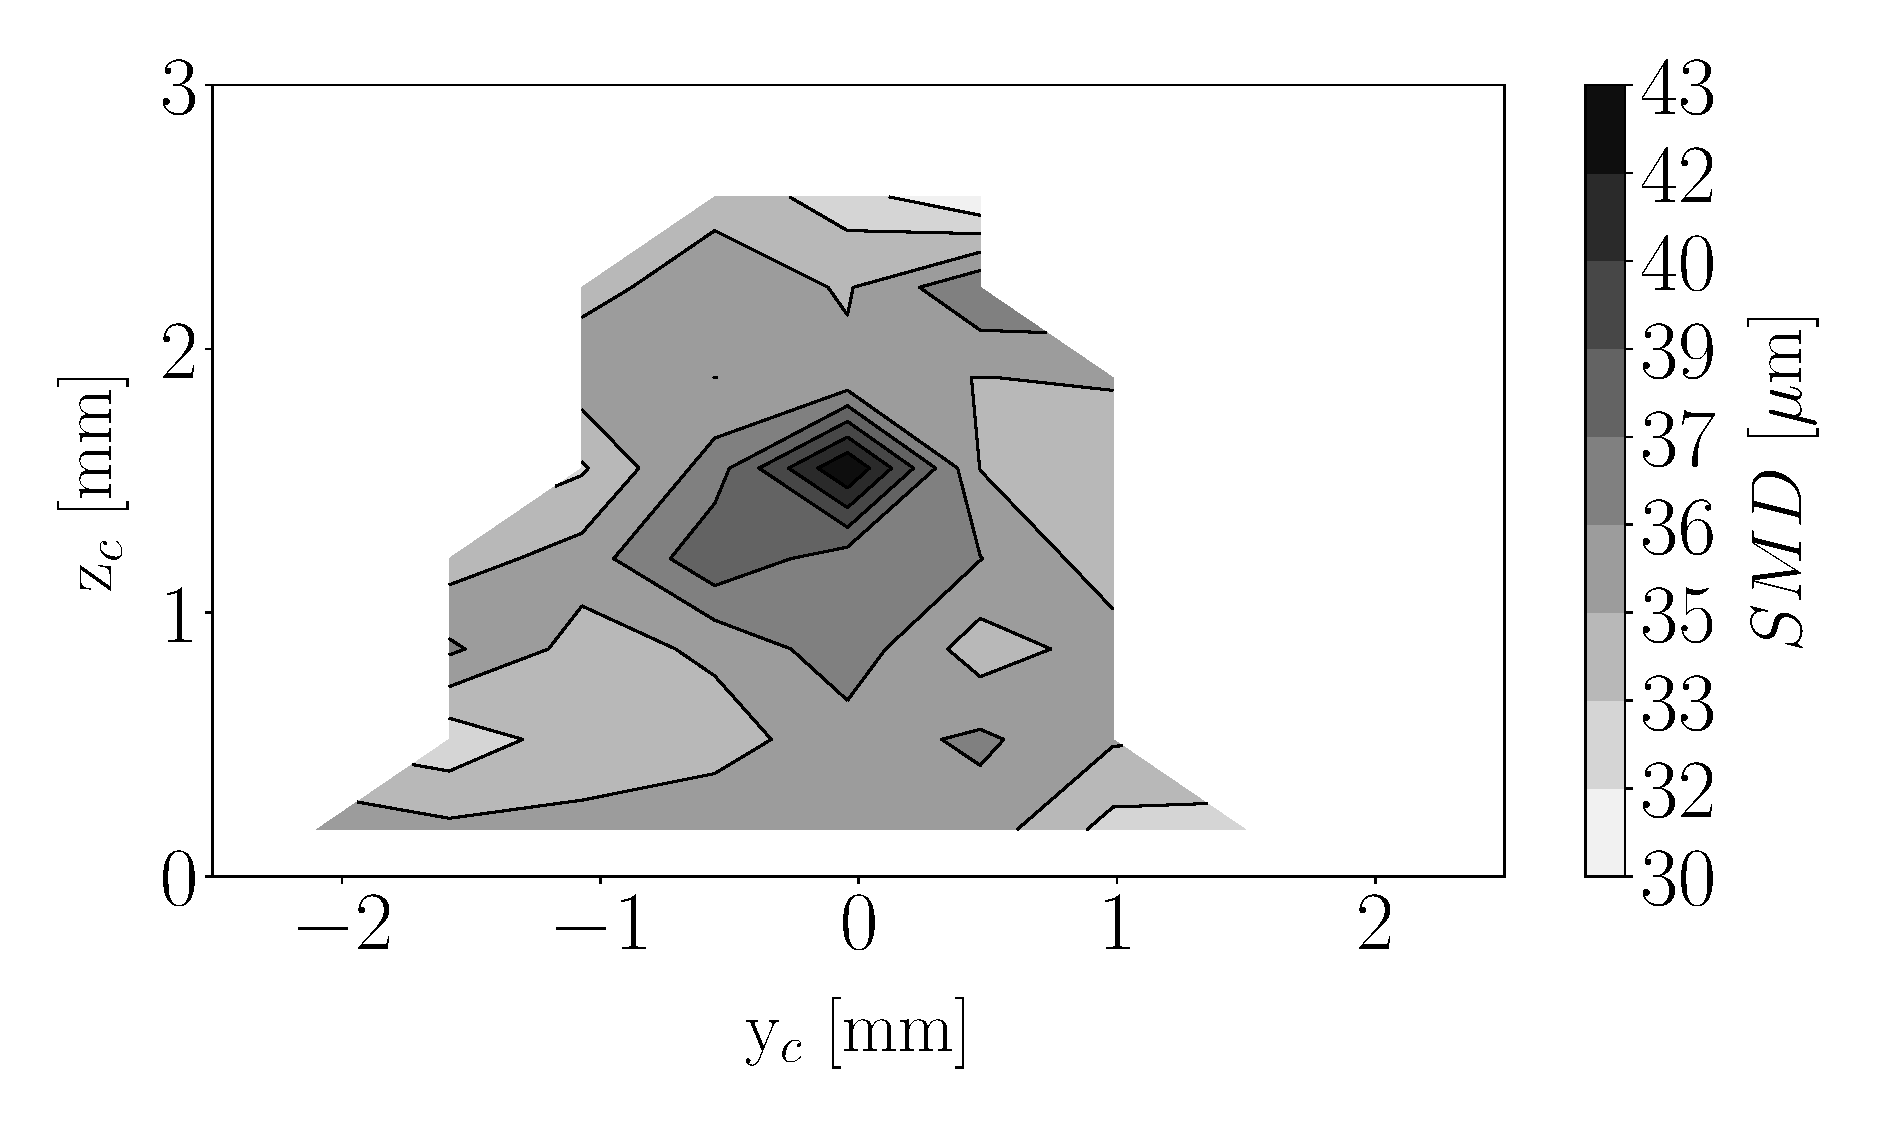
\includegraphics[scale=\scaleSLIBIMER]{./part3_applications/figures_ch8_resolved/injectors_SLI/dx10_xD05p00_SMD_map}
   %\caption{Case UG100\_DX20: crossflow planes}
   %\label{} 
\end{subfigure}
   \hspace{0.17in}
\begin{subfigure}[b]{0.3\textwidth}
	\centering
   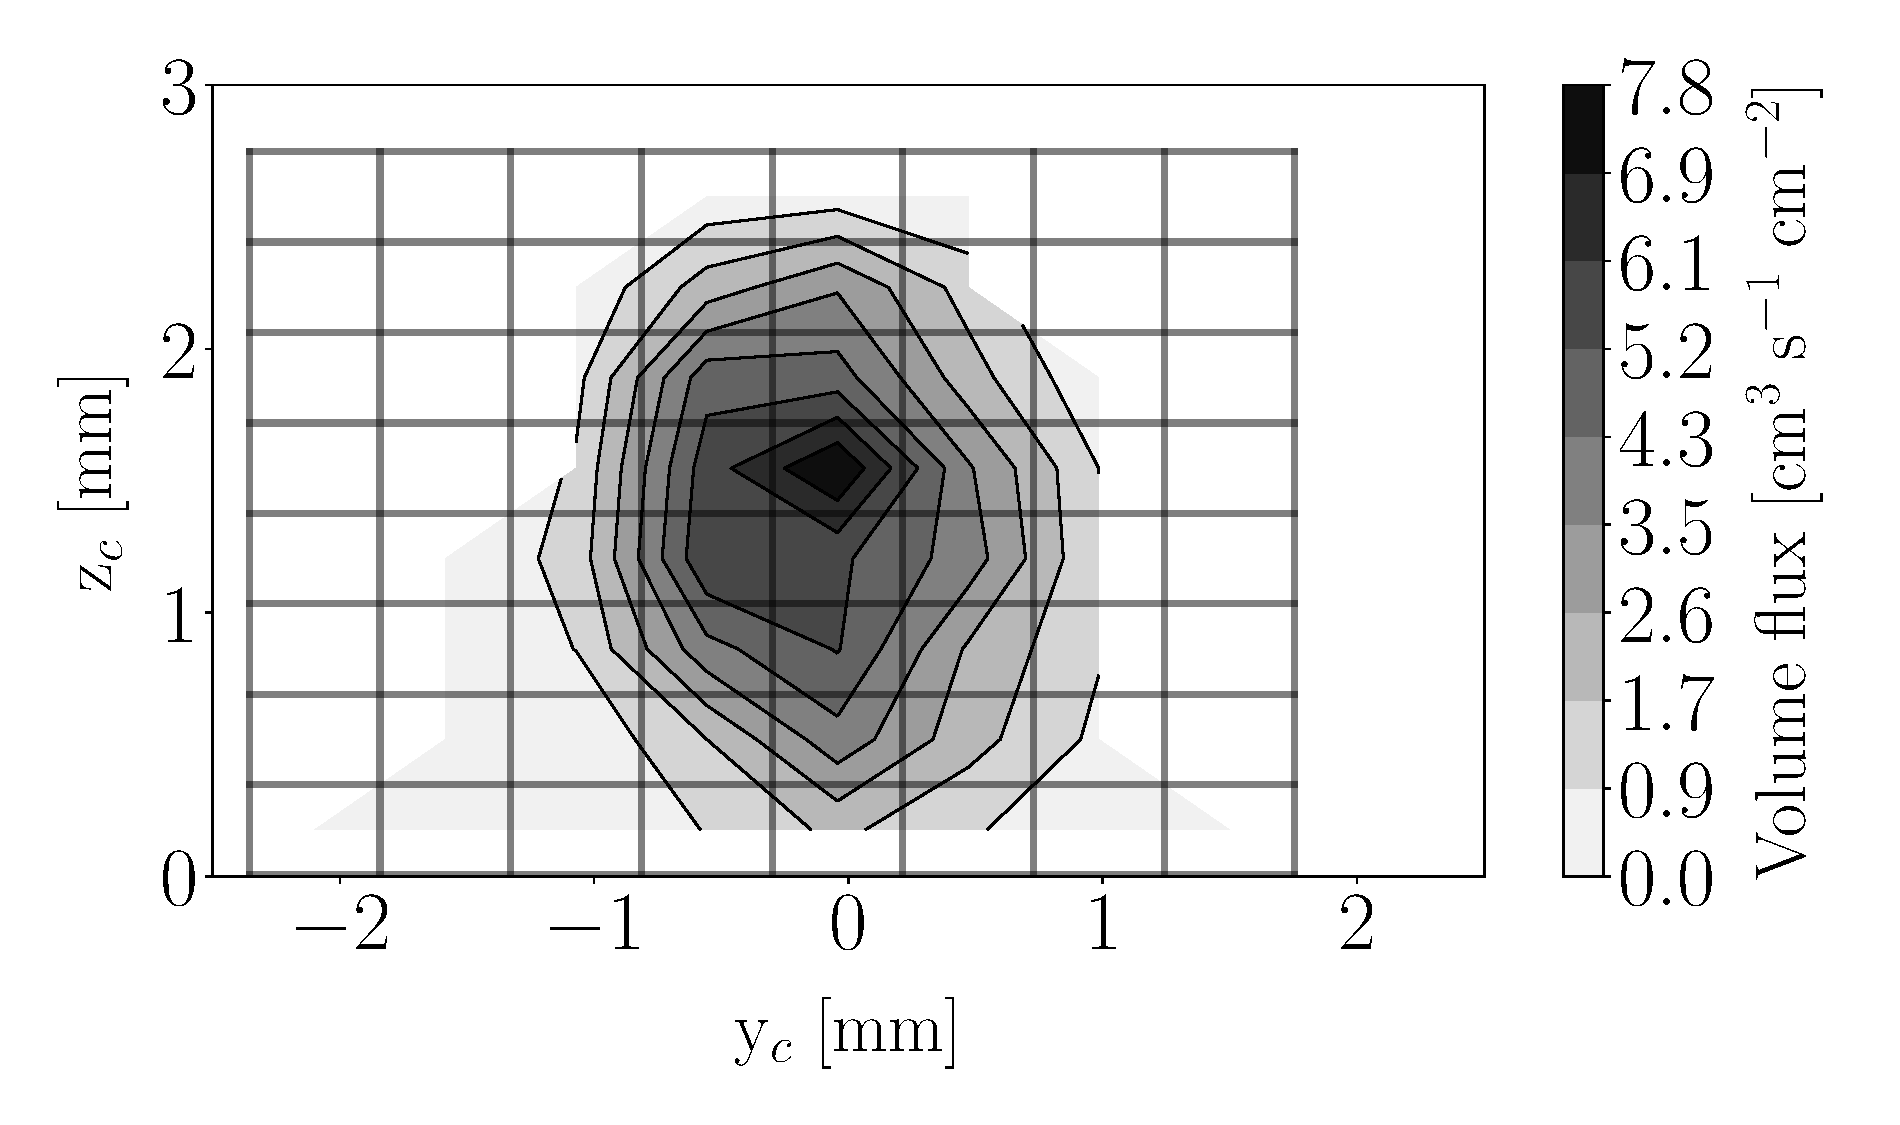
\includegraphics[scale=\scaleSLIBIMER]{./part3_applications/figures_ch8_resolved/injectors_SLI/dx10_xD05p00_volume_flux_map}
   %\caption{Case UG100\_DX20: filming planes}
   %\label{}
\end{subfigure}
   \hspace{0.17in}
\begin{subfigure}[b]{0.3\textwidth}
	\centering
   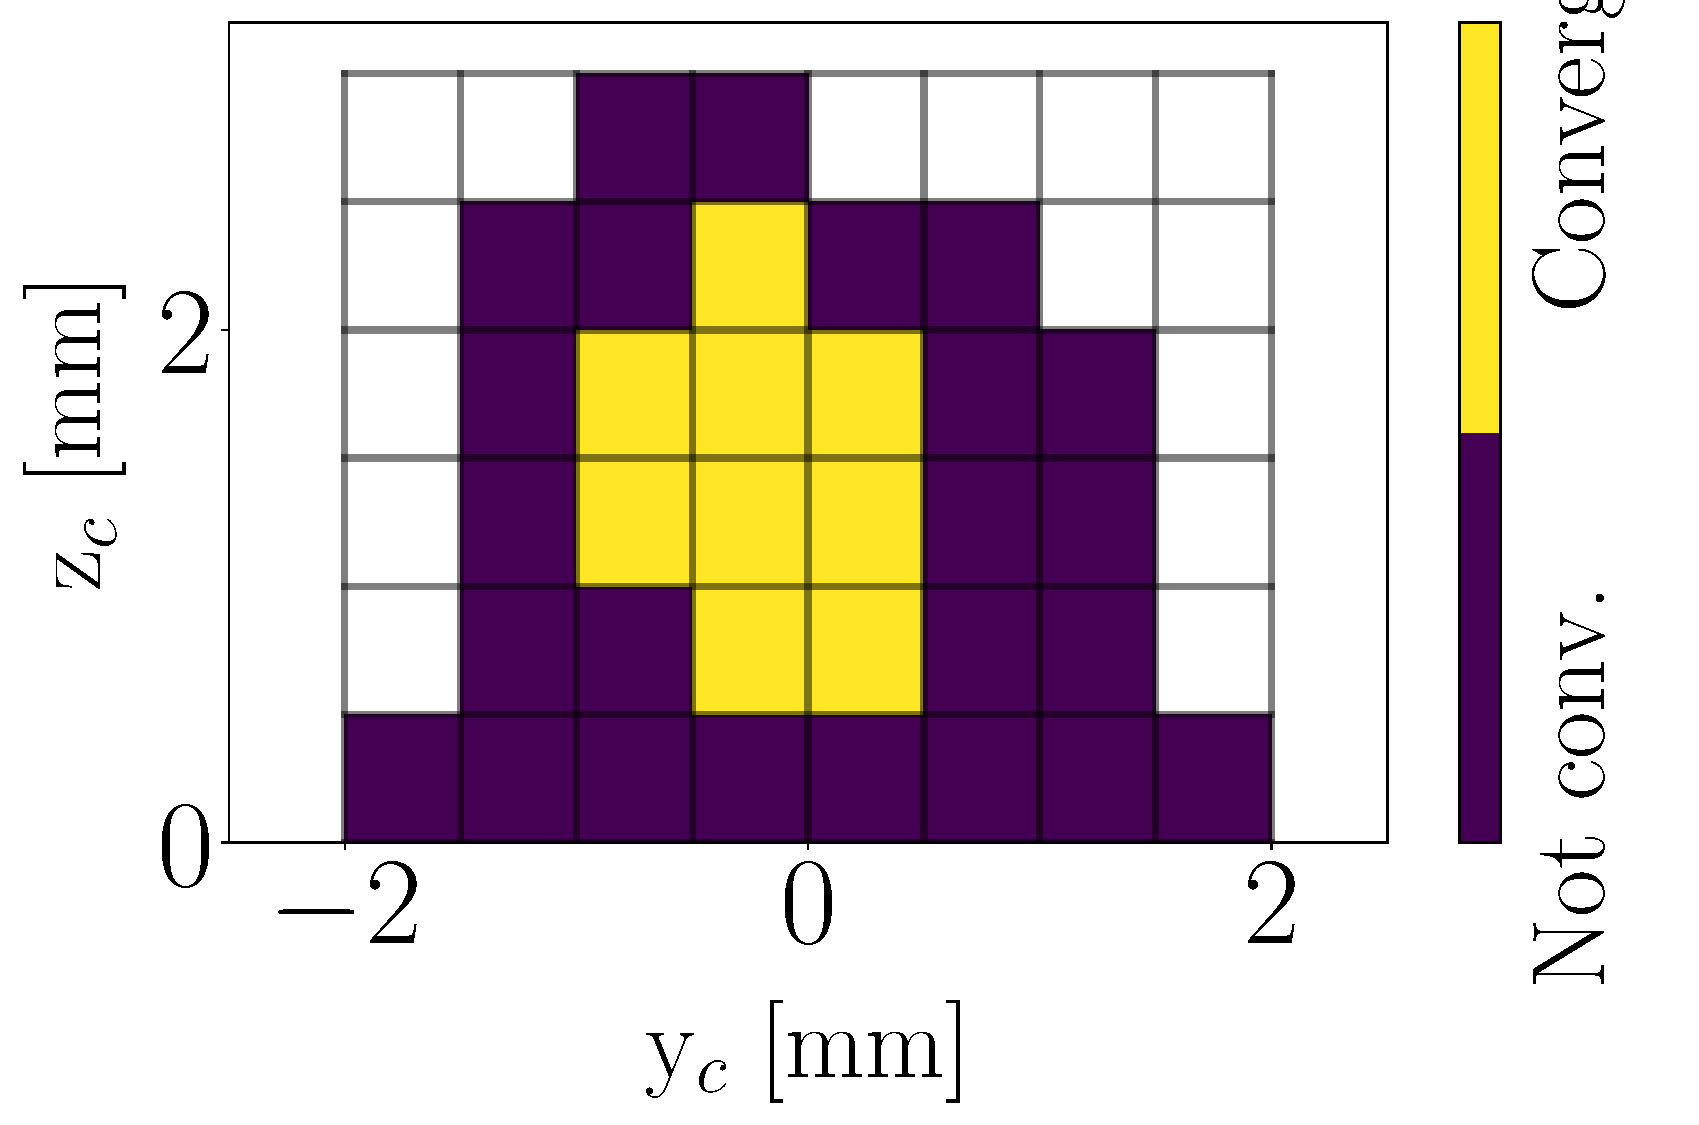
\includegraphics[scale=\scaleSLIBIMER]{./part3_applications/figures_ch8_resolved/injectors_SLI/dx10_xD05p00_convergence_map}
   %\caption{Case UG100\_DX10: crossflow planes}
   %\label{} 
\end{subfigure}

\vskip\baselineskip

\begin{subfigure}[b]{0.3\textwidth}
	\centering
   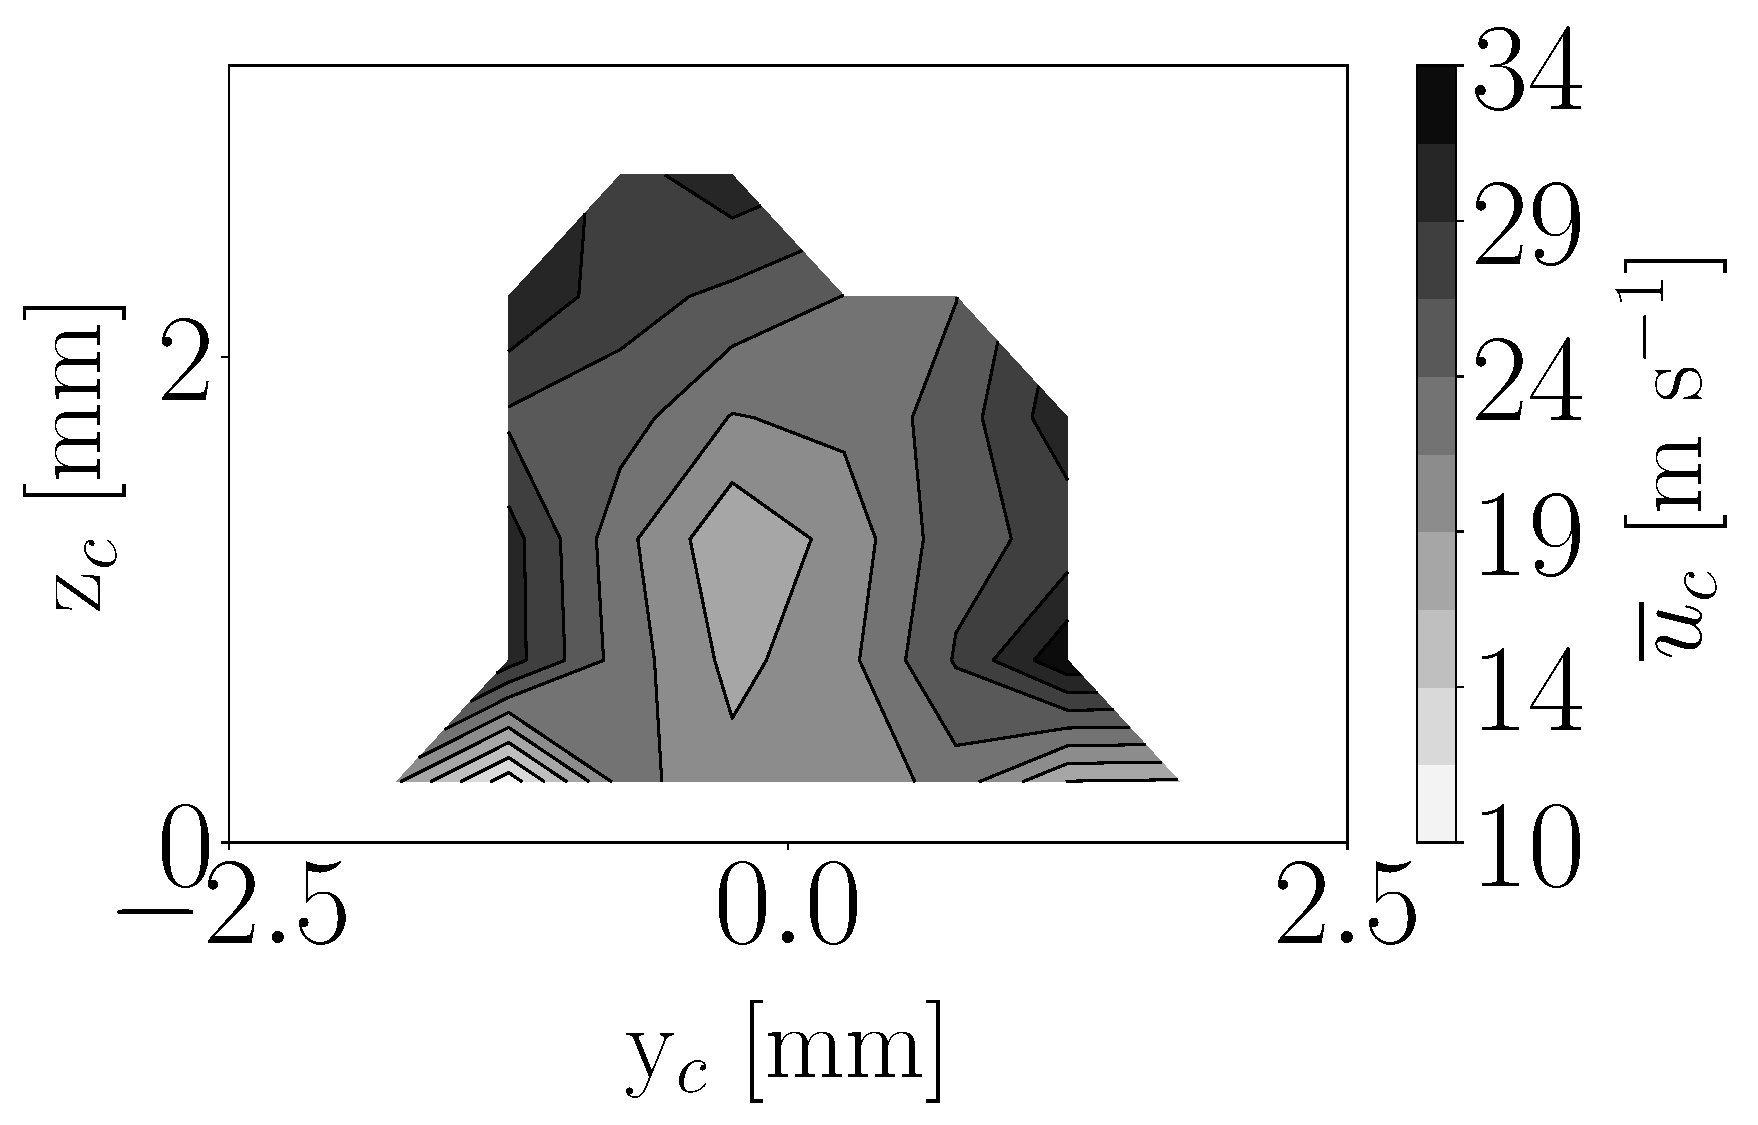
\includegraphics[scale=\scaleSLIBIMER]{./part3_applications/figures_ch8_resolved/injectors_SLI/dx10_xD05p00_ux_mean_map}
   %\caption{Case UG100\_DX20: crossflow planes}
   %\label{} 
\end{subfigure}
   \hspace{0.17in}
\begin{subfigure}[b]{0.3\textwidth}
	\centering
   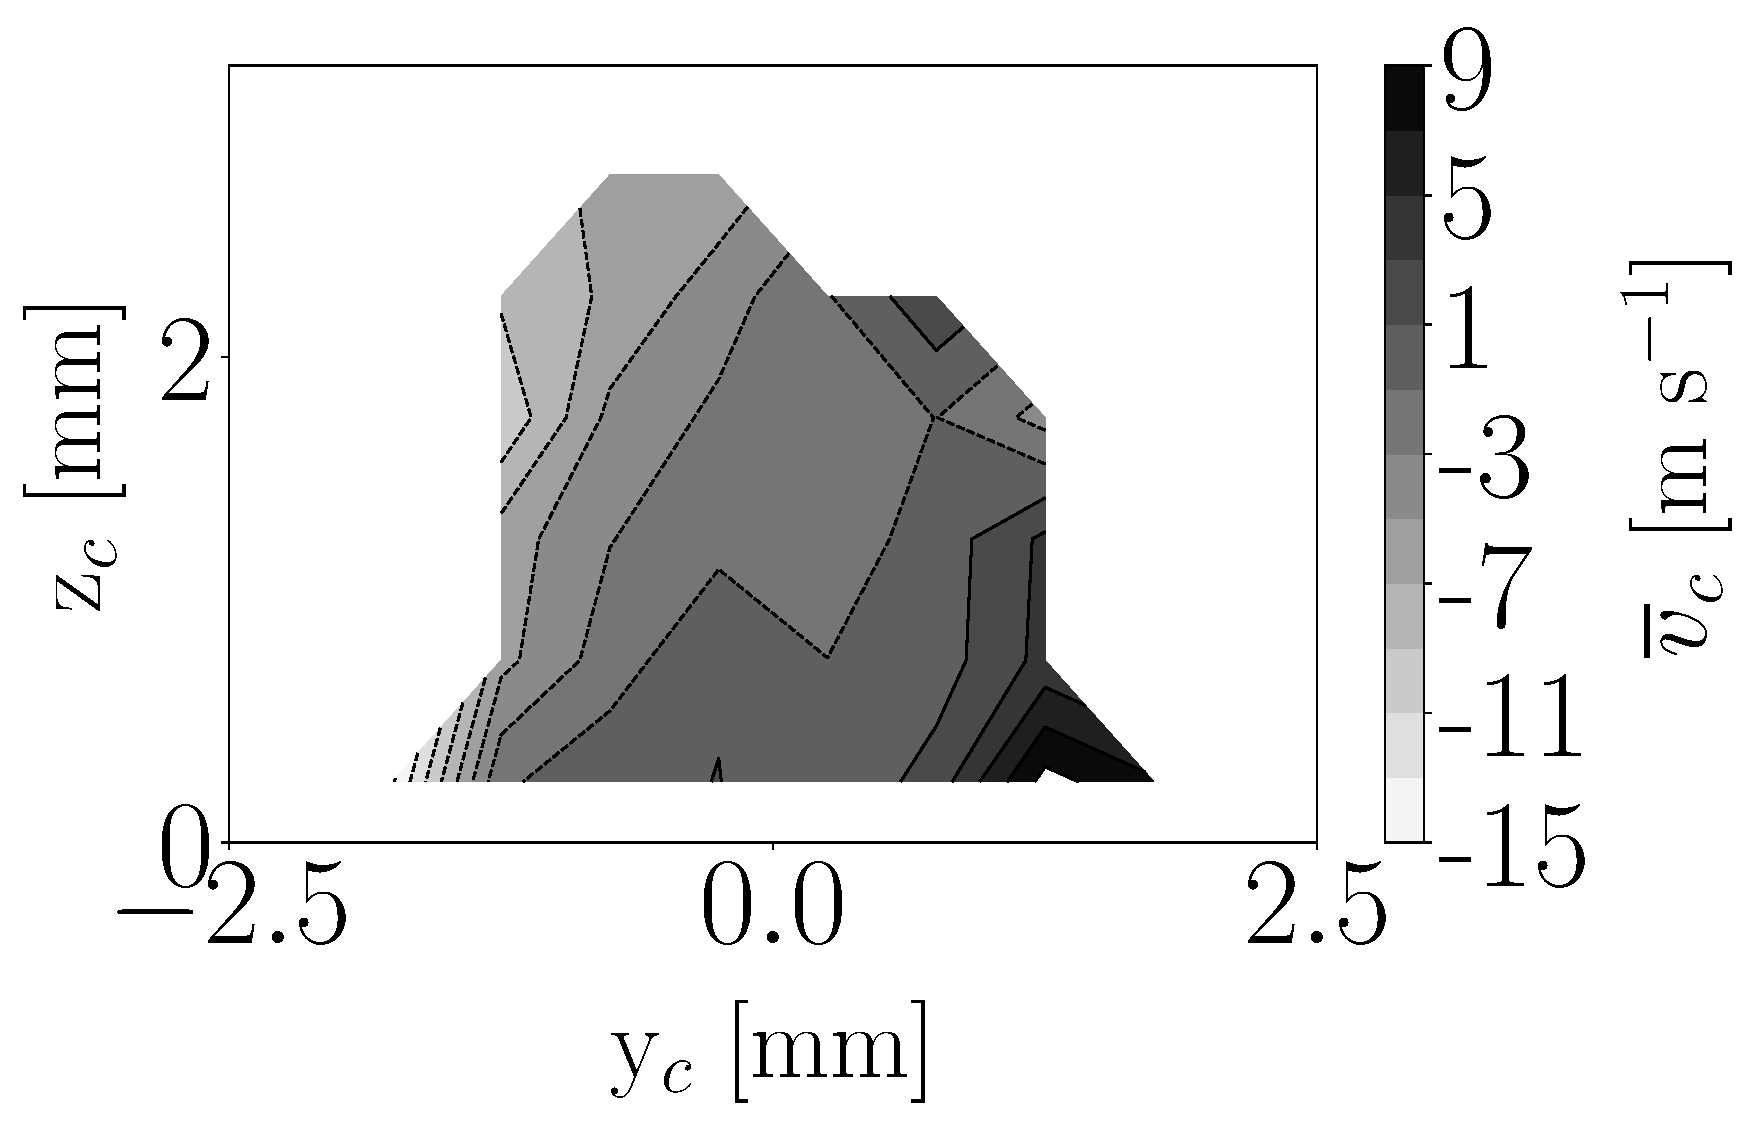
\includegraphics[scale=\scaleSLIBIMER]{./part3_applications/figures_ch8_resolved/injectors_SLI/dx10_xD05p00_uy_mean_map}
   %\caption{Case UG100\_DX20: filming planes}
   %\label{}
\end{subfigure}
   \hspace{0.17in}
\begin{subfigure}[b]{0.3\textwidth}
	\centering
   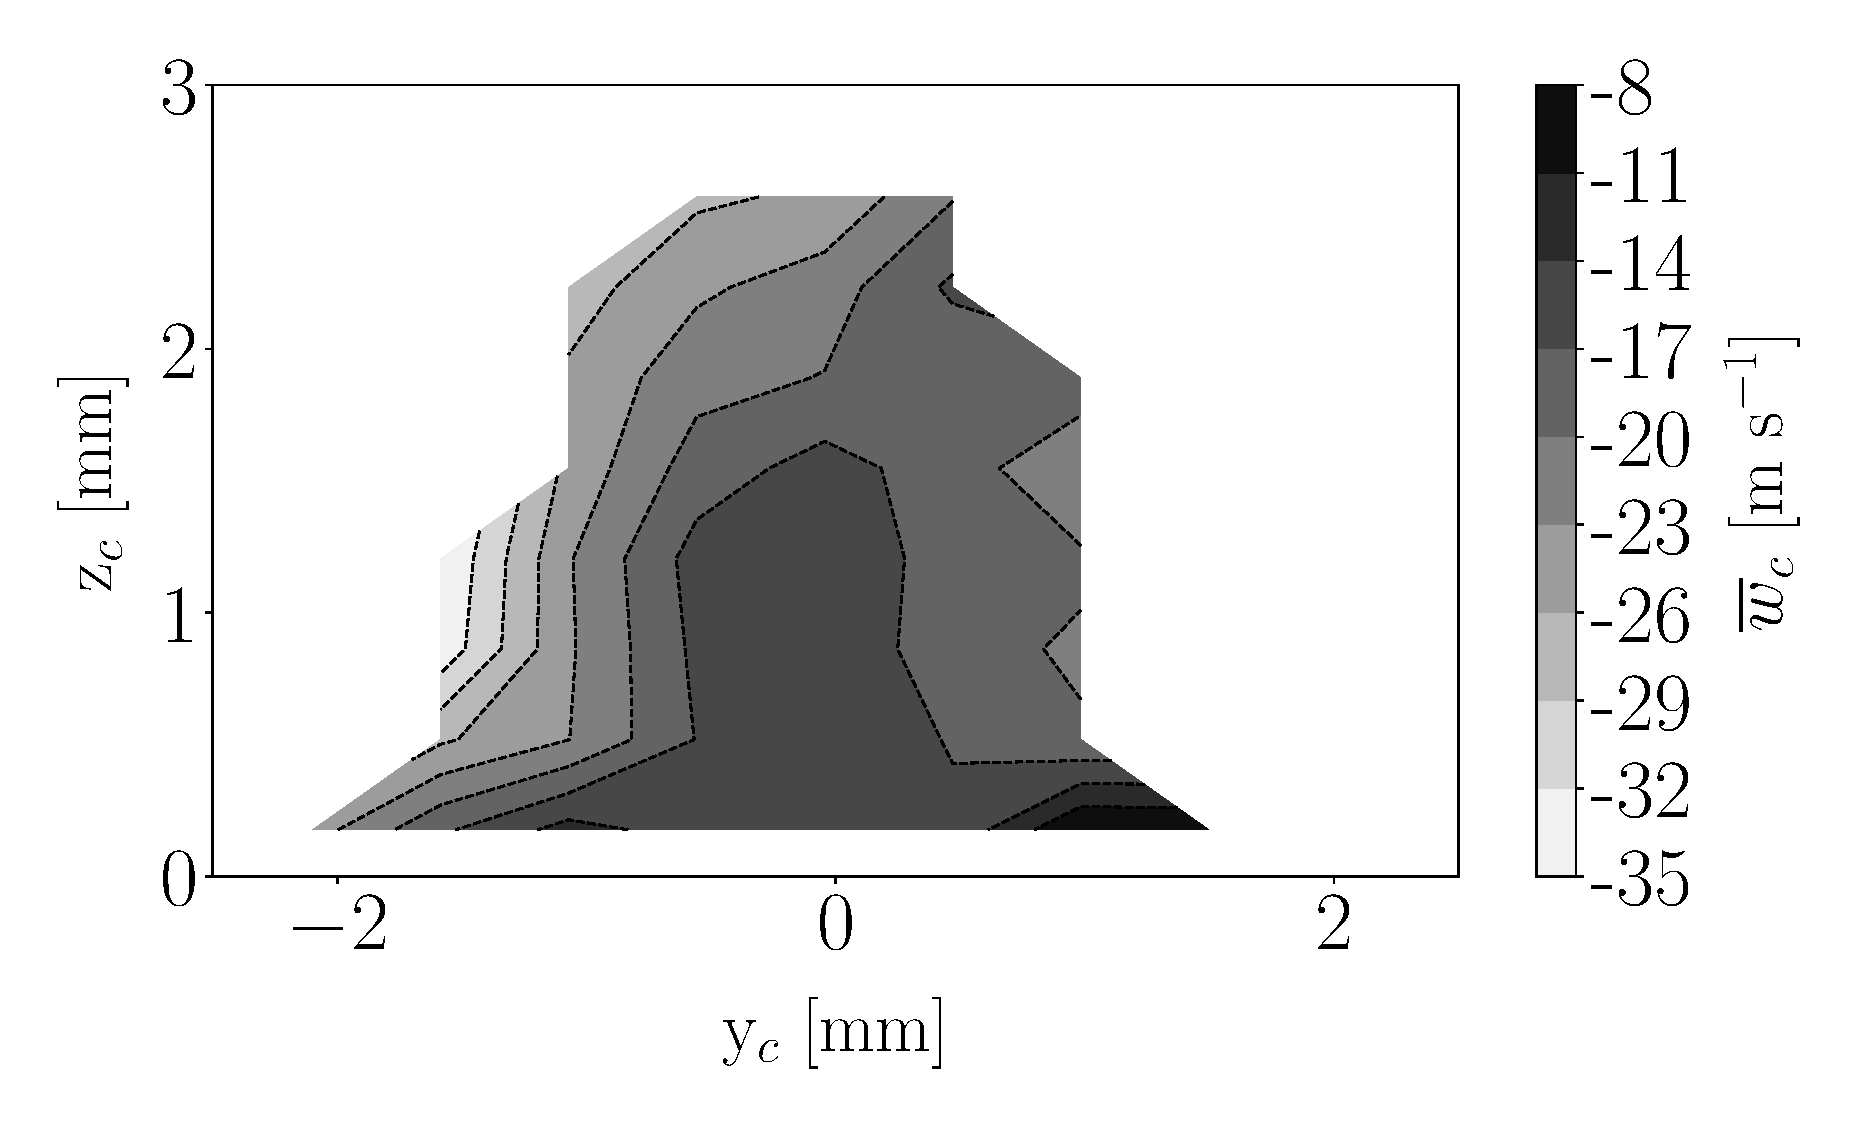
\includegraphics[scale=\scaleSLIBIMER]{./part3_applications/figures_ch8_resolved/injectors_SLI/dx10_xD05p00_uz_mean_map}
   %\caption{Case UG100\_DX10: crossflow planes}
   %\label{} 
\end{subfigure}
\caption{Spray states at $x_c$ = 1.5 mm for case DX10}
%\caption{Spray states at $x/d_\mathrm{inj}$ = 5 for case DX10}
\label{fig:injectors_sli_BIMER_DX10_xD05}
\end{figure}


%%%%%%%%%%%%%%%% DX10, xD = 6.67


\begin{figure}[h!]
\centering
\begin{subfigure}[b]{0.3\textwidth}
	\centering
   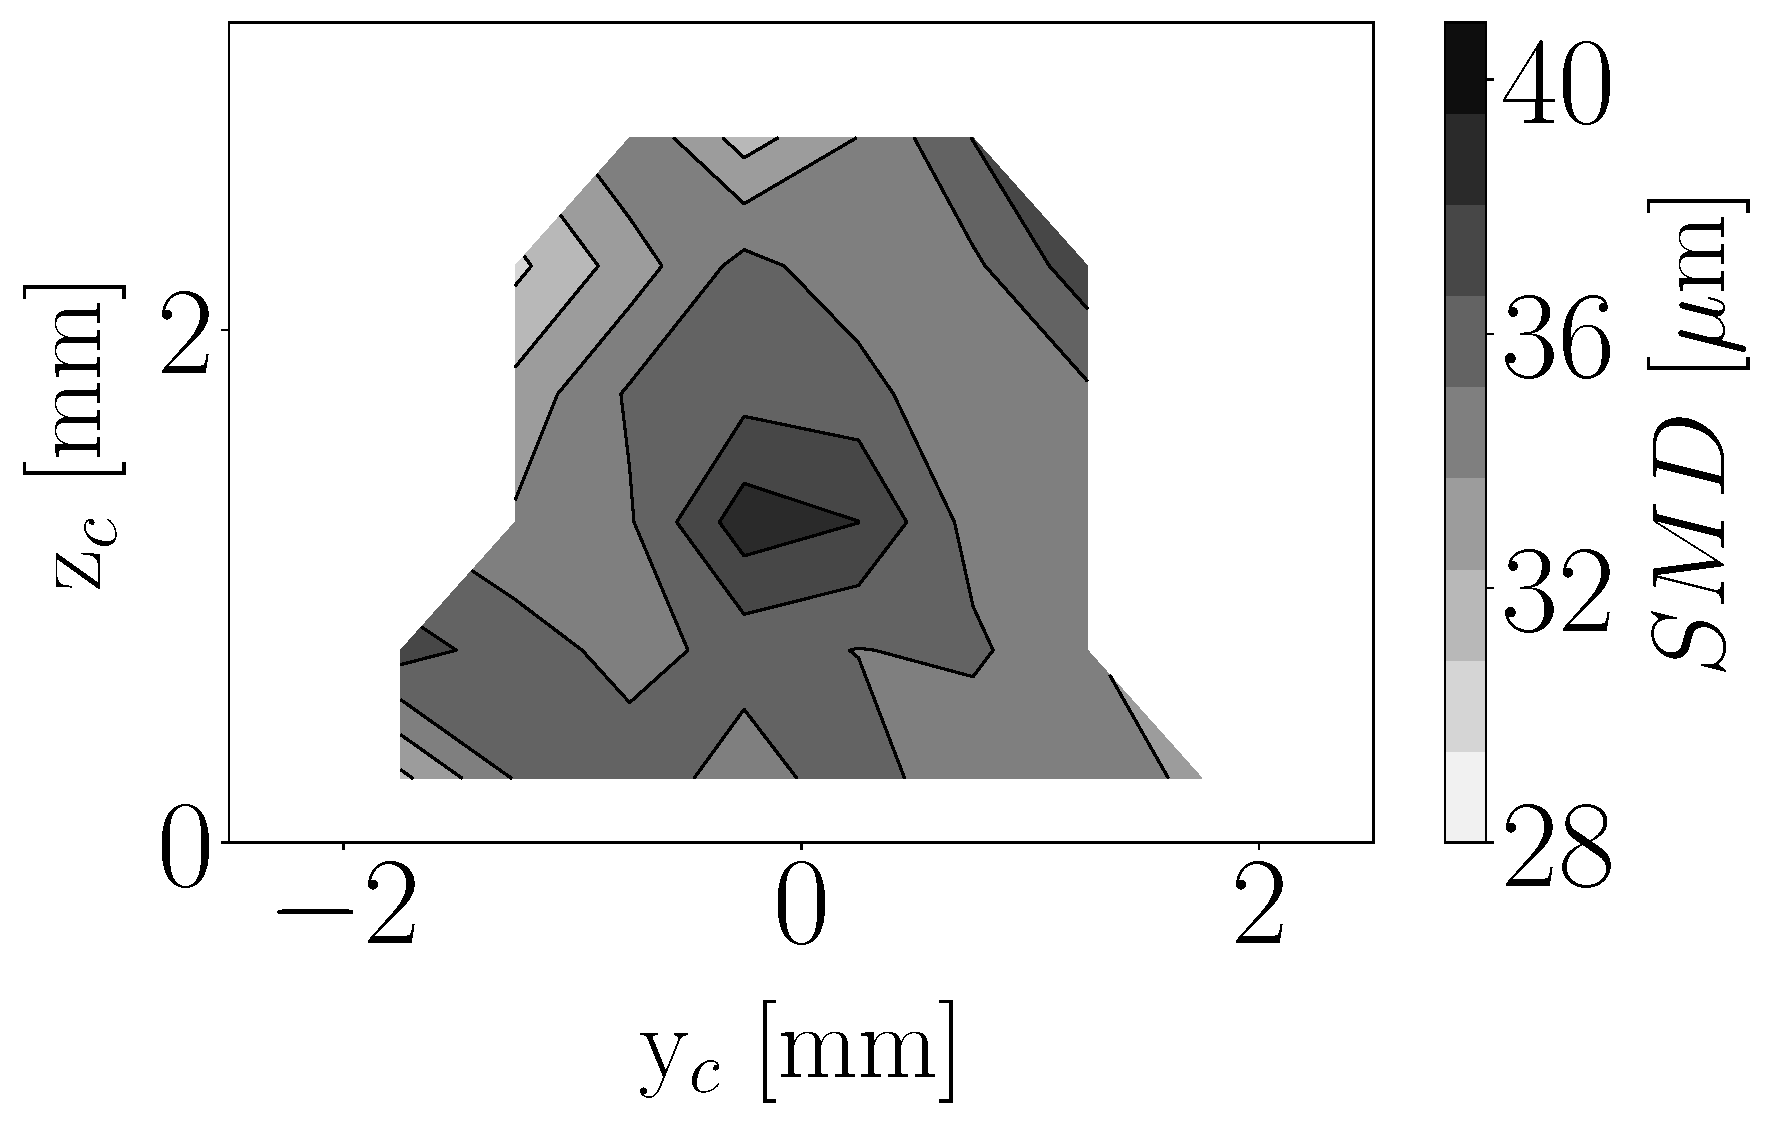
\includegraphics[scale=\scaleSLIBIMER]{./part3_applications/figures_ch8_resolved/injectors_SLI/dx10_xD06p67_SMD_map}
   %\caption{Case UG100\_DX20: crossflow planes}
   %\label{} 
\end{subfigure}
   \hspace{0.17in}
\begin{subfigure}[b]{0.3\textwidth}
	\centering
   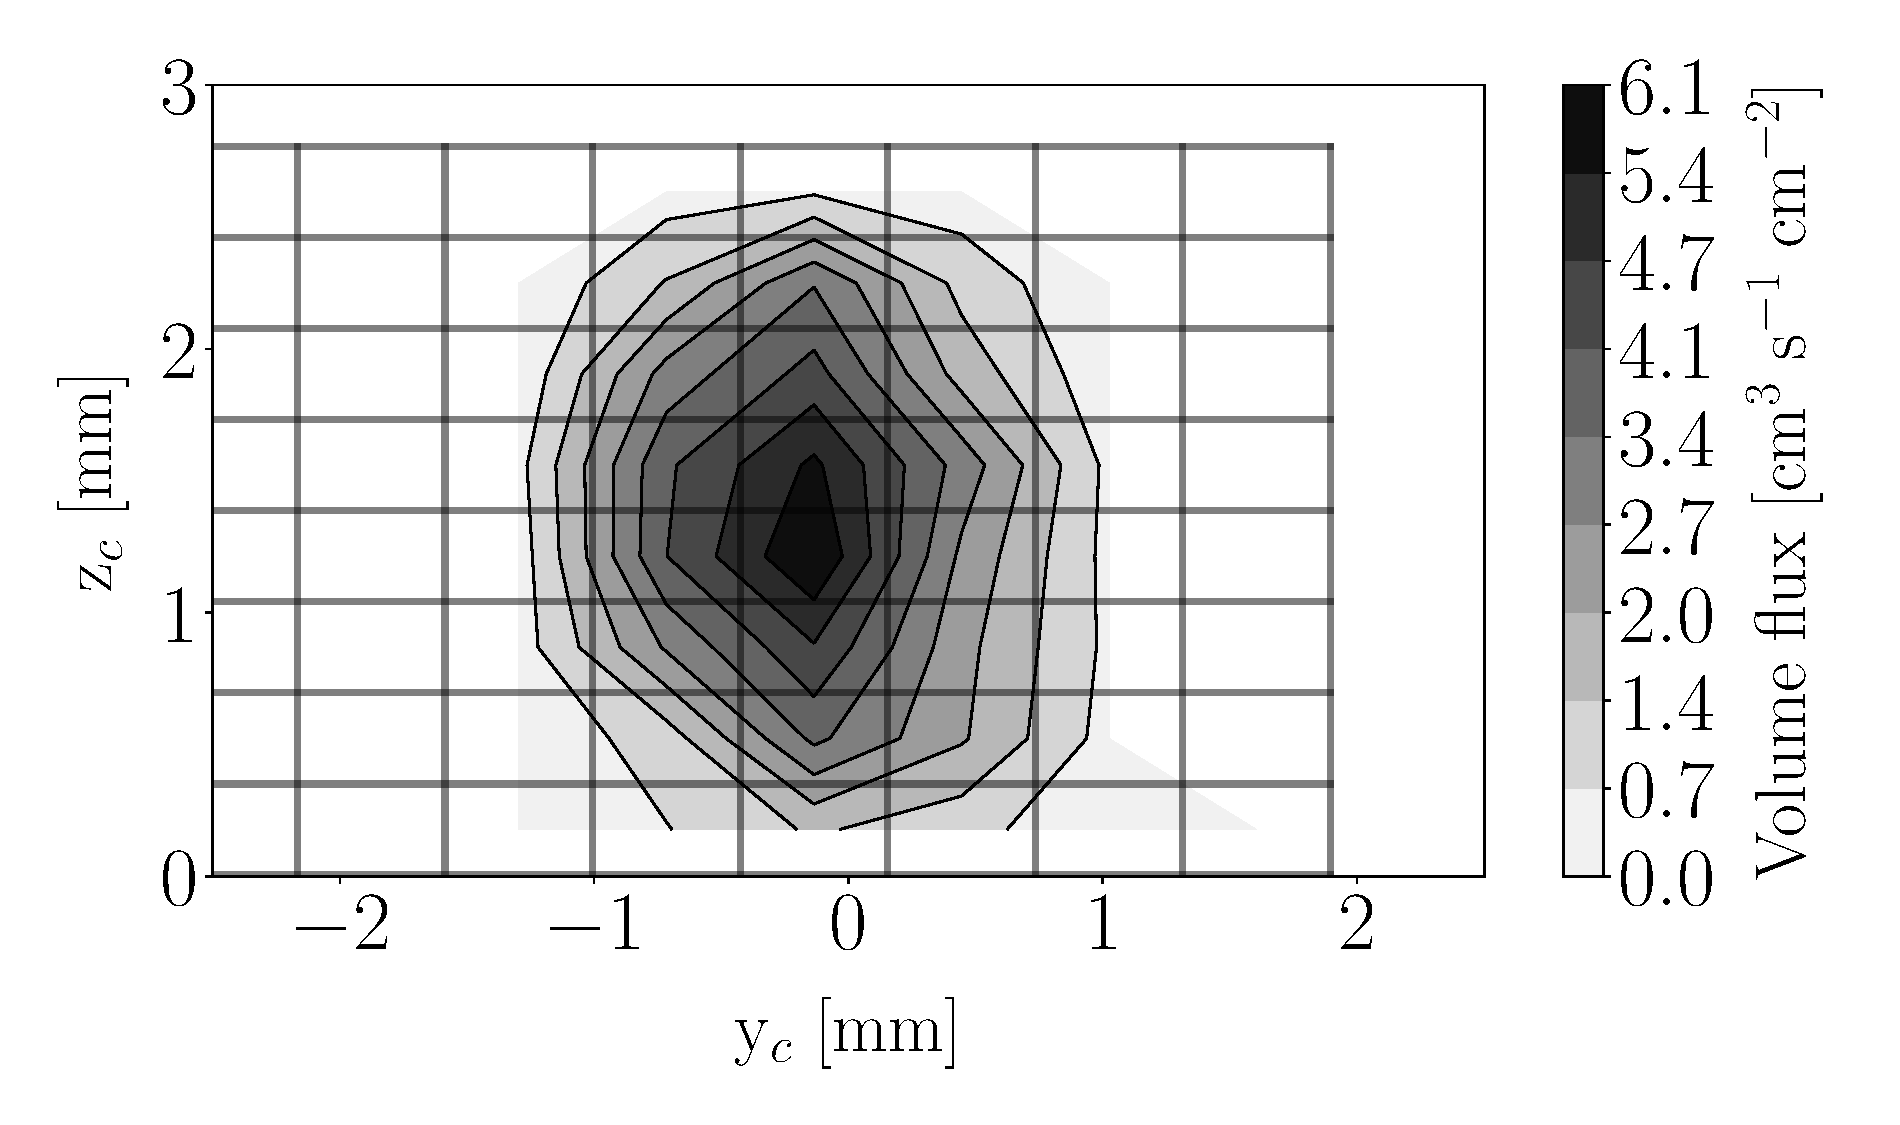
\includegraphics[scale=\scaleSLIBIMER]{./part3_applications/figures_ch8_resolved/injectors_SLI/dx10_xD06p67_volume_flux_map}
   %\caption{Case UG100\_DX20: filming planes}
   %\label{}
\end{subfigure}
   \hspace{0.17in}
\begin{subfigure}[b]{0.3\textwidth}
	\centering
   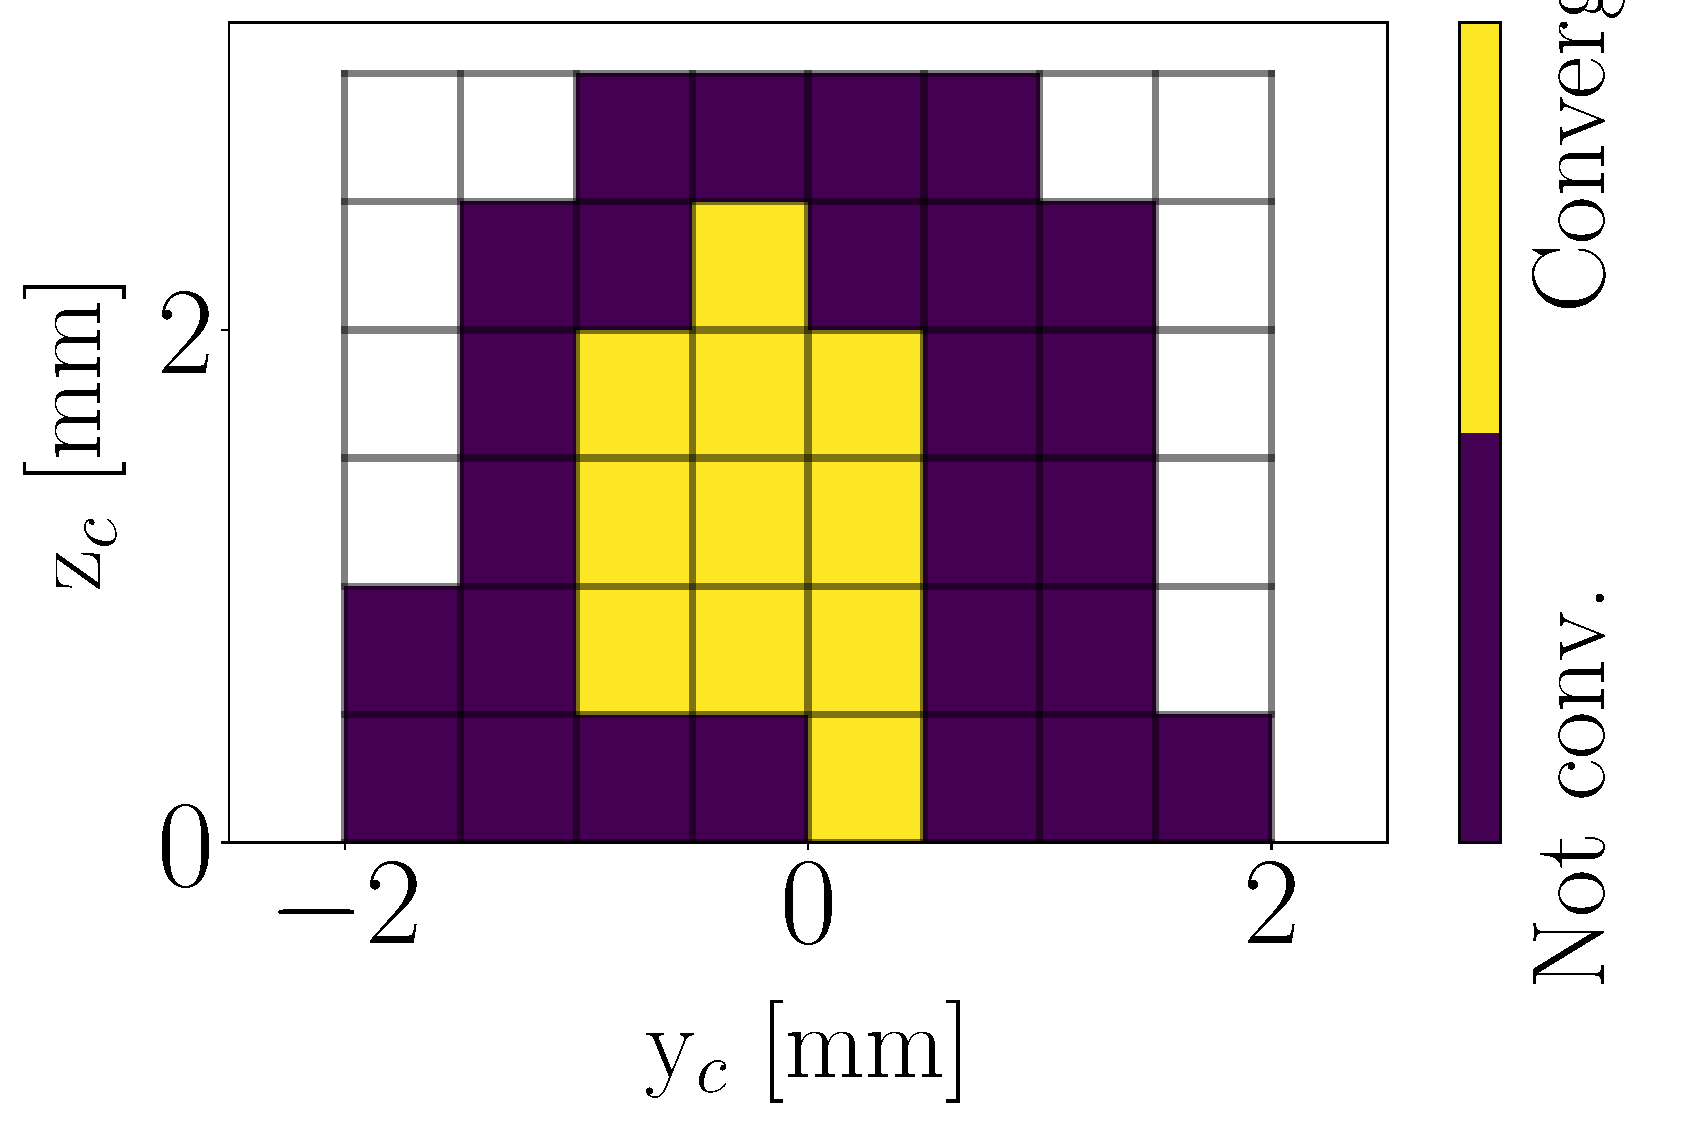
\includegraphics[scale=\scaleSLIBIMER]{./part3_applications/figures_ch8_resolved/injectors_SLI/dx10_xD06p67_convergence_map}
   %\caption{Case UG100\_DX10: crossflow planes}
   %\label{} 
\end{subfigure}

\vskip\baselineskip

\begin{subfigure}[b]{0.3\textwidth}
	\centering
   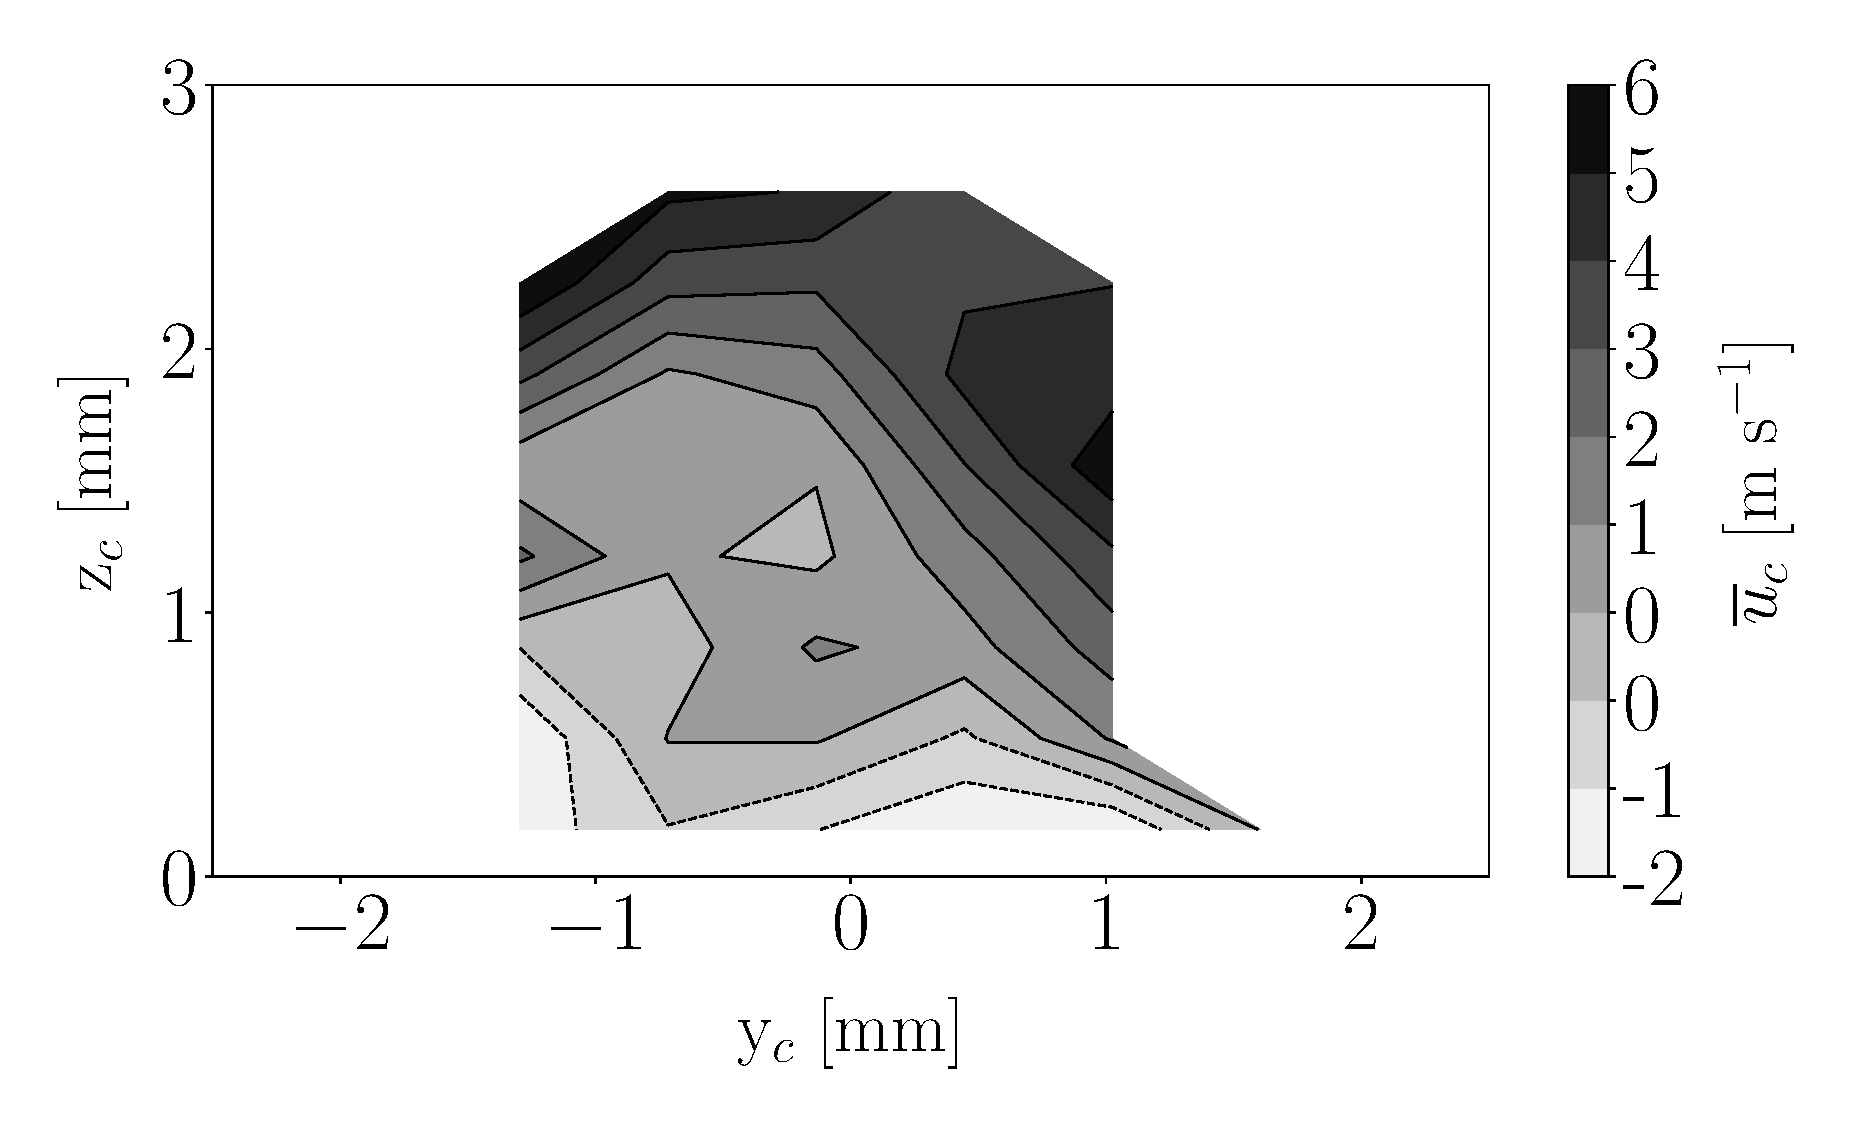
\includegraphics[scale=\scaleSLIBIMER]{./part3_applications/figures_ch8_resolved/injectors_SLI/dx10_xD06p67_ux_mean_map}
   %\caption{Case UG100\_DX20: crossflow planes}
   %\label{} 
\end{subfigure}
   \hspace{0.17in}
\begin{subfigure}[b]{0.3\textwidth}
	\centering
   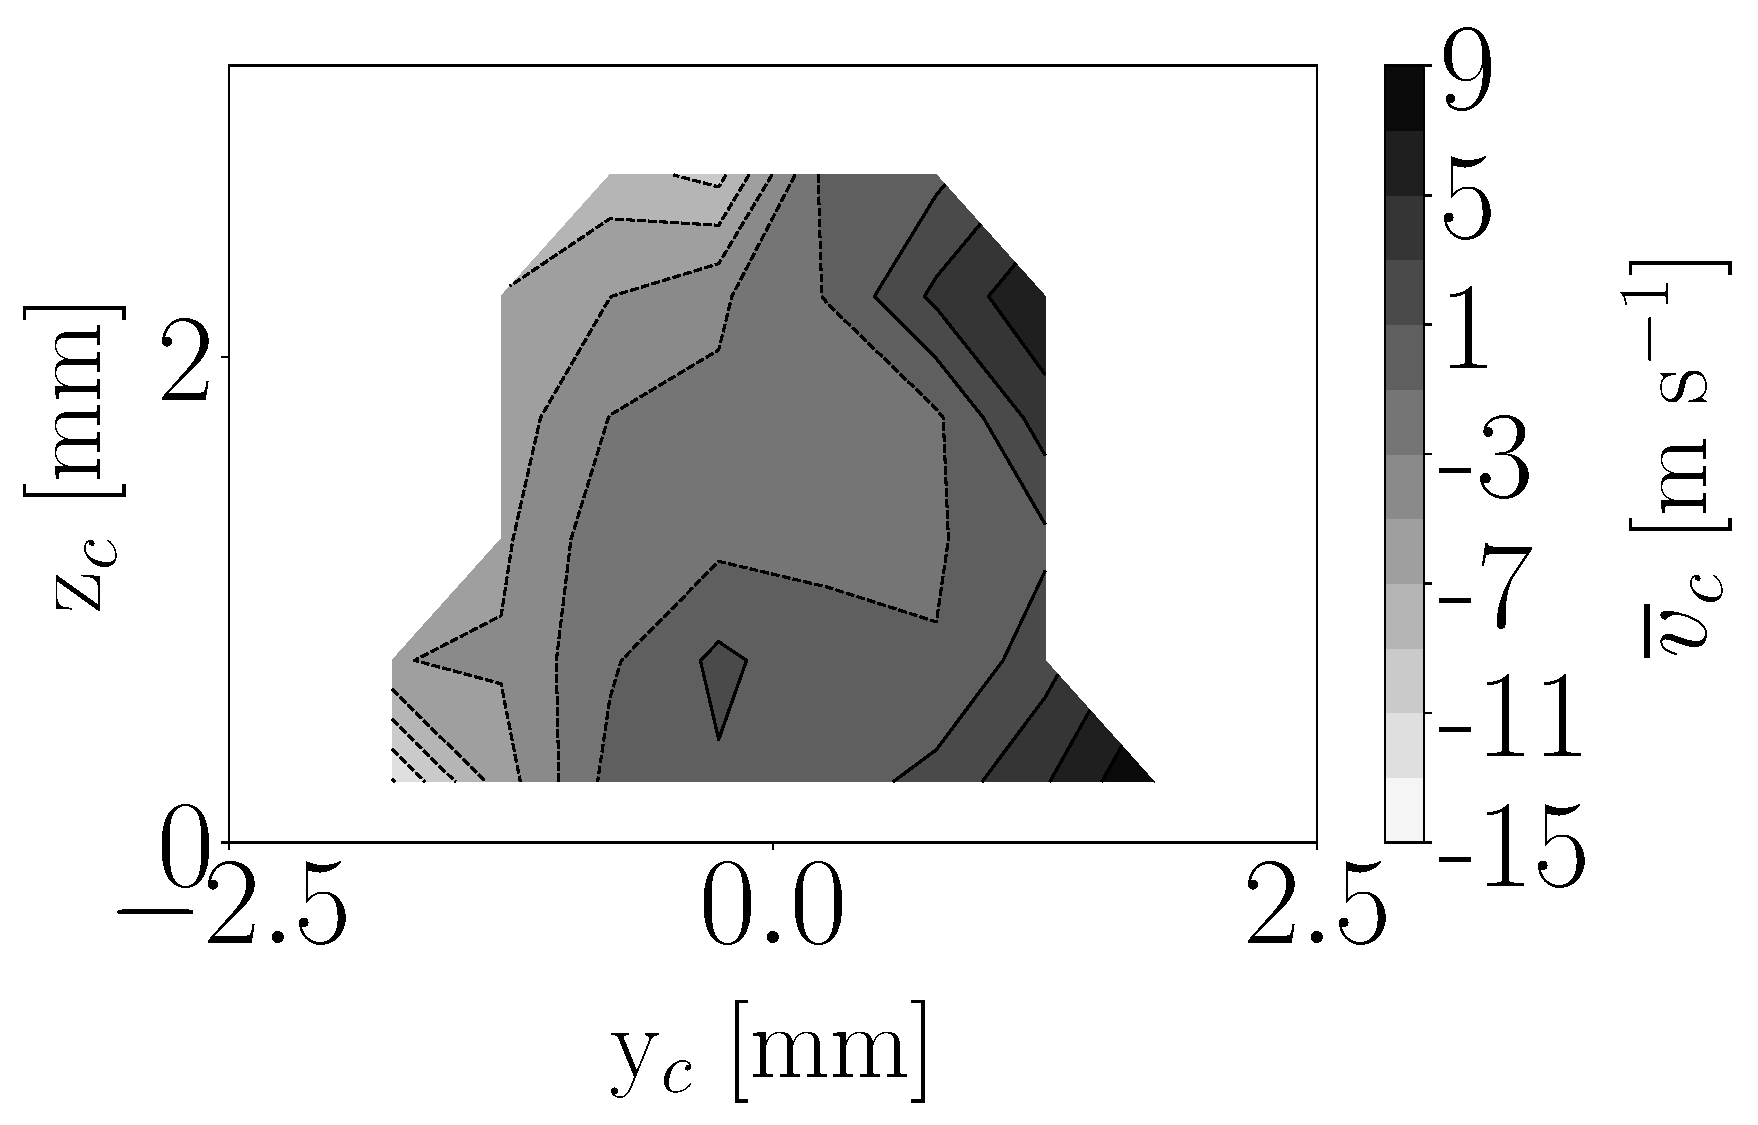
\includegraphics[scale=\scaleSLIBIMER]{./part3_applications/figures_ch8_resolved/injectors_SLI/dx10_xD06p67_uy_mean_map}
   %\caption{Case UG100\_DX20: filming planes}
   %\label{}
\end{subfigure}
   \hspace{0.17in}
\begin{subfigure}[b]{0.3\textwidth}
	\centering
   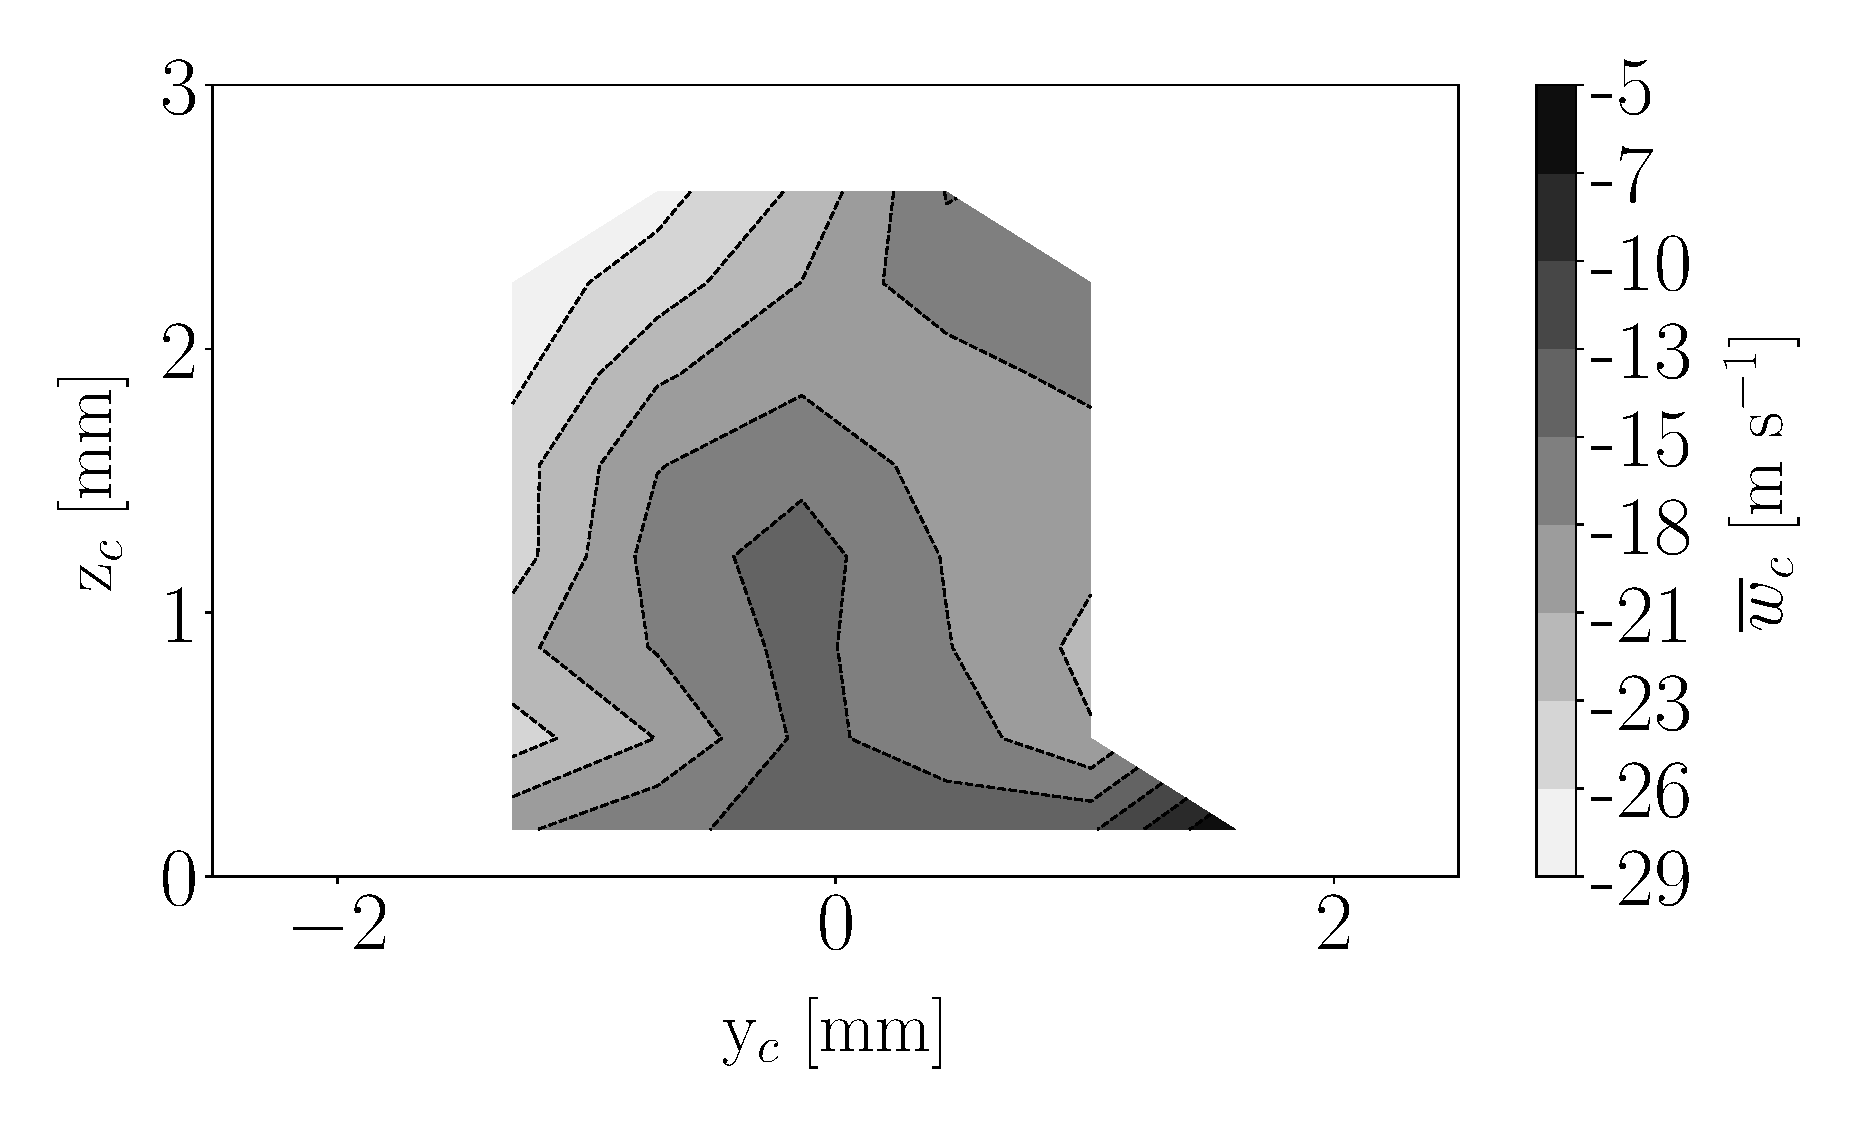
\includegraphics[scale=\scaleSLIBIMER]{./part3_applications/figures_ch8_resolved/injectors_SLI/dx10_xD06p67_uz_mean_map}
   %\caption{Case UG100\_DX10: crossflow planes}
   %\label{} 
\end{subfigure}
\caption{Spray states at $x_c$ = 2 mm for case DX10}
%\caption{Spray states at $x/d_\mathrm{inj}$ = 6.67 for case DX10}
\label{fig:injectors_sli_BIMER_DX10_xD06p67}
\end{figure}


\clearpage

\subsubsection*{Case DX15}



%%%%%%%%%%%%%%%% DX15, xD = 5


\begin{figure}[h!]
\centering
\begin{subfigure}[b]{0.3\textwidth}
	\centering
   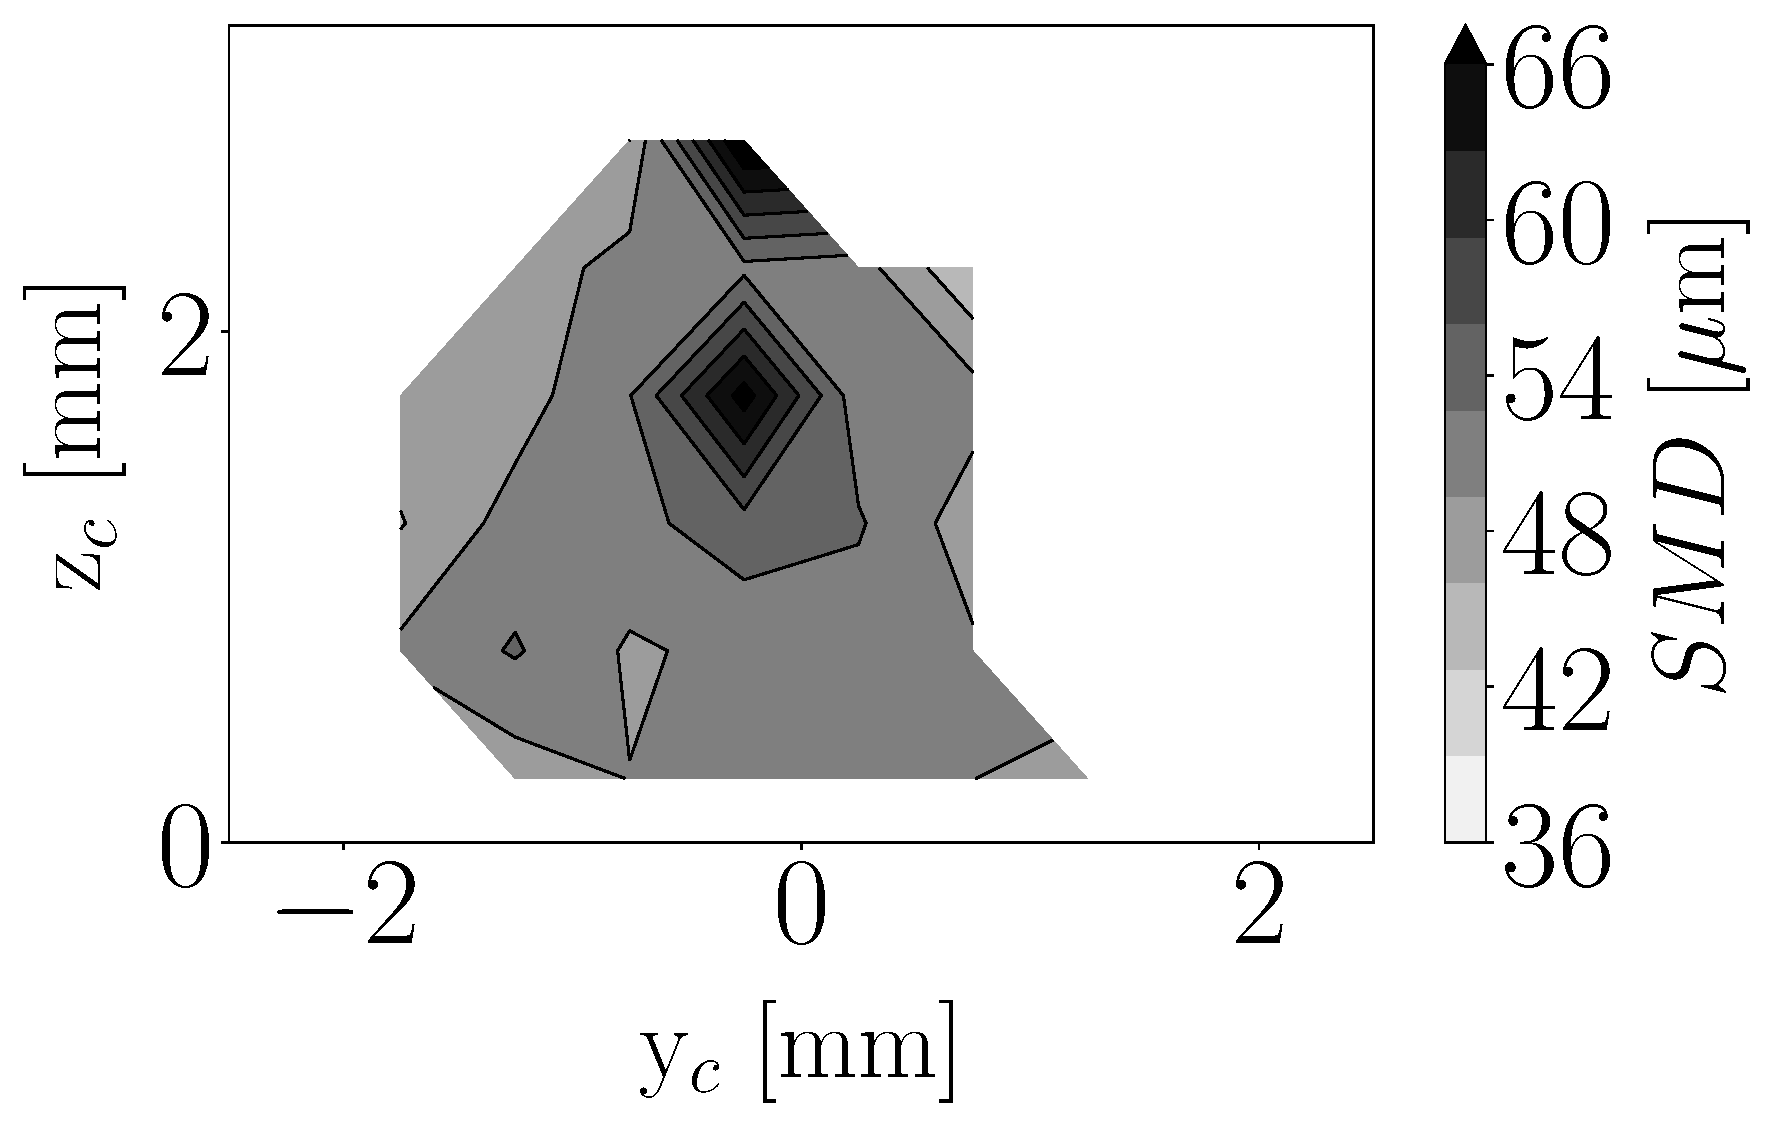
\includegraphics[scale=\scaleSLIBIMER]{./part3_applications/figures_ch8_resolved/injectors_SLI/dx15_xD05p00_SMD_map}
   %\caption{Case UG100\_DX20: crossflow planes}
   %\label{} 
\end{subfigure}
   \hspace{0.17in}
\begin{subfigure}[b]{0.3\textwidth}
	\centering
   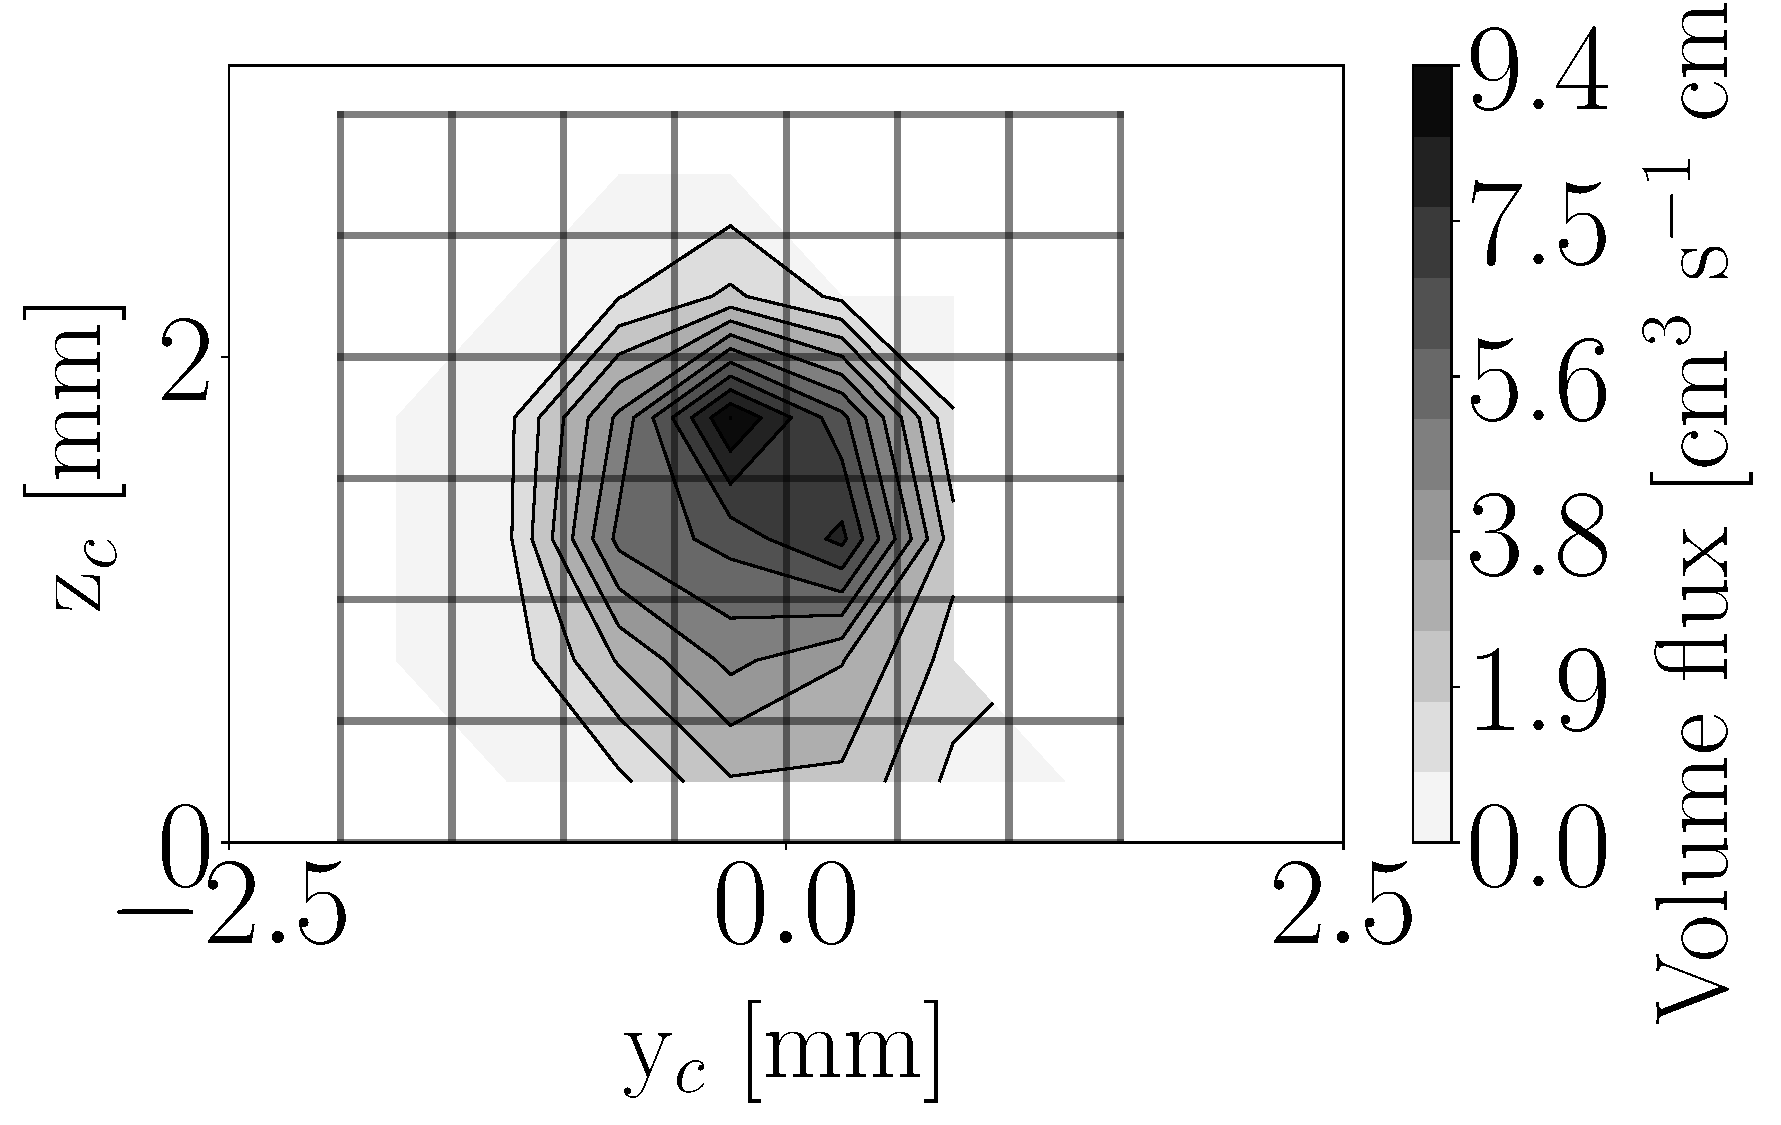
\includegraphics[scale=\scaleSLIBIMER]{./part3_applications/figures_ch8_resolved/injectors_SLI/dx15_xD05p00_volume_flux_map}
   %\caption{Case UG100\_DX20: filming planes}
   %\label{}
\end{subfigure}
   \hspace{0.17in}
\begin{subfigure}[b]{0.3\textwidth}
	\centering
   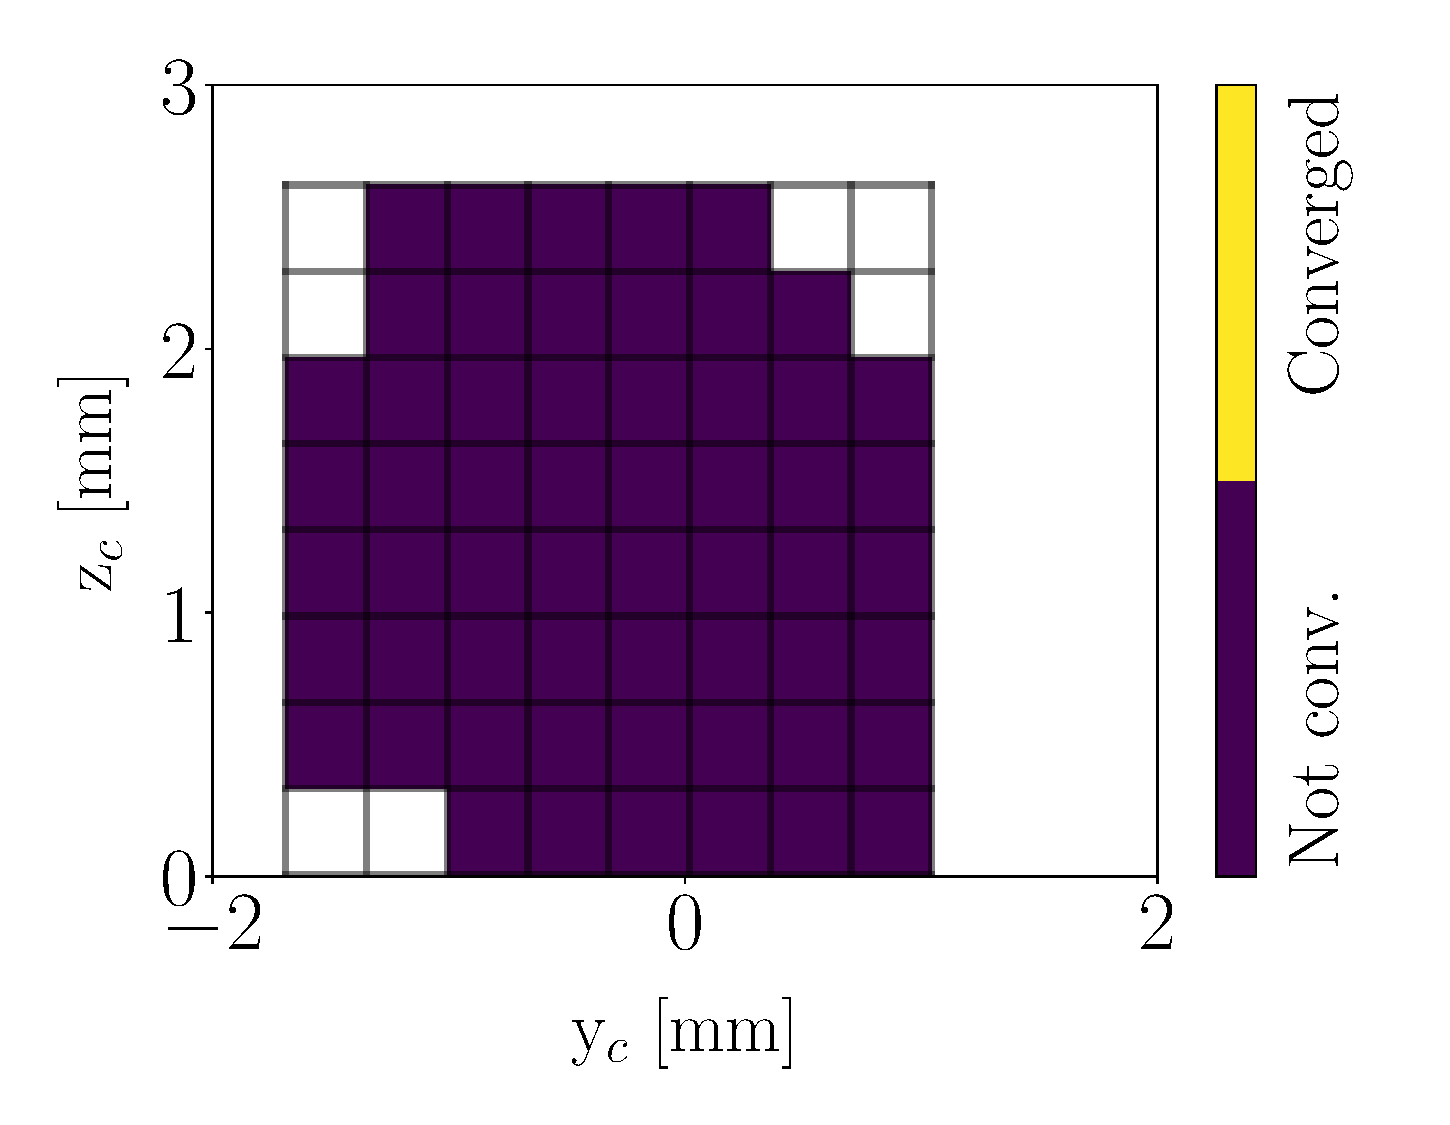
\includegraphics[scale=\scaleSLIBIMER]{./part3_applications/figures_ch8_resolved/injectors_SLI/dx15_xD05p00_convergence_map}
   %\caption{Case UG100\_DX10: crossflow planes}
   %\label{} 
\end{subfigure}

\vskip\baselineskip

\begin{subfigure}[b]{0.3\textwidth}
	\centering
   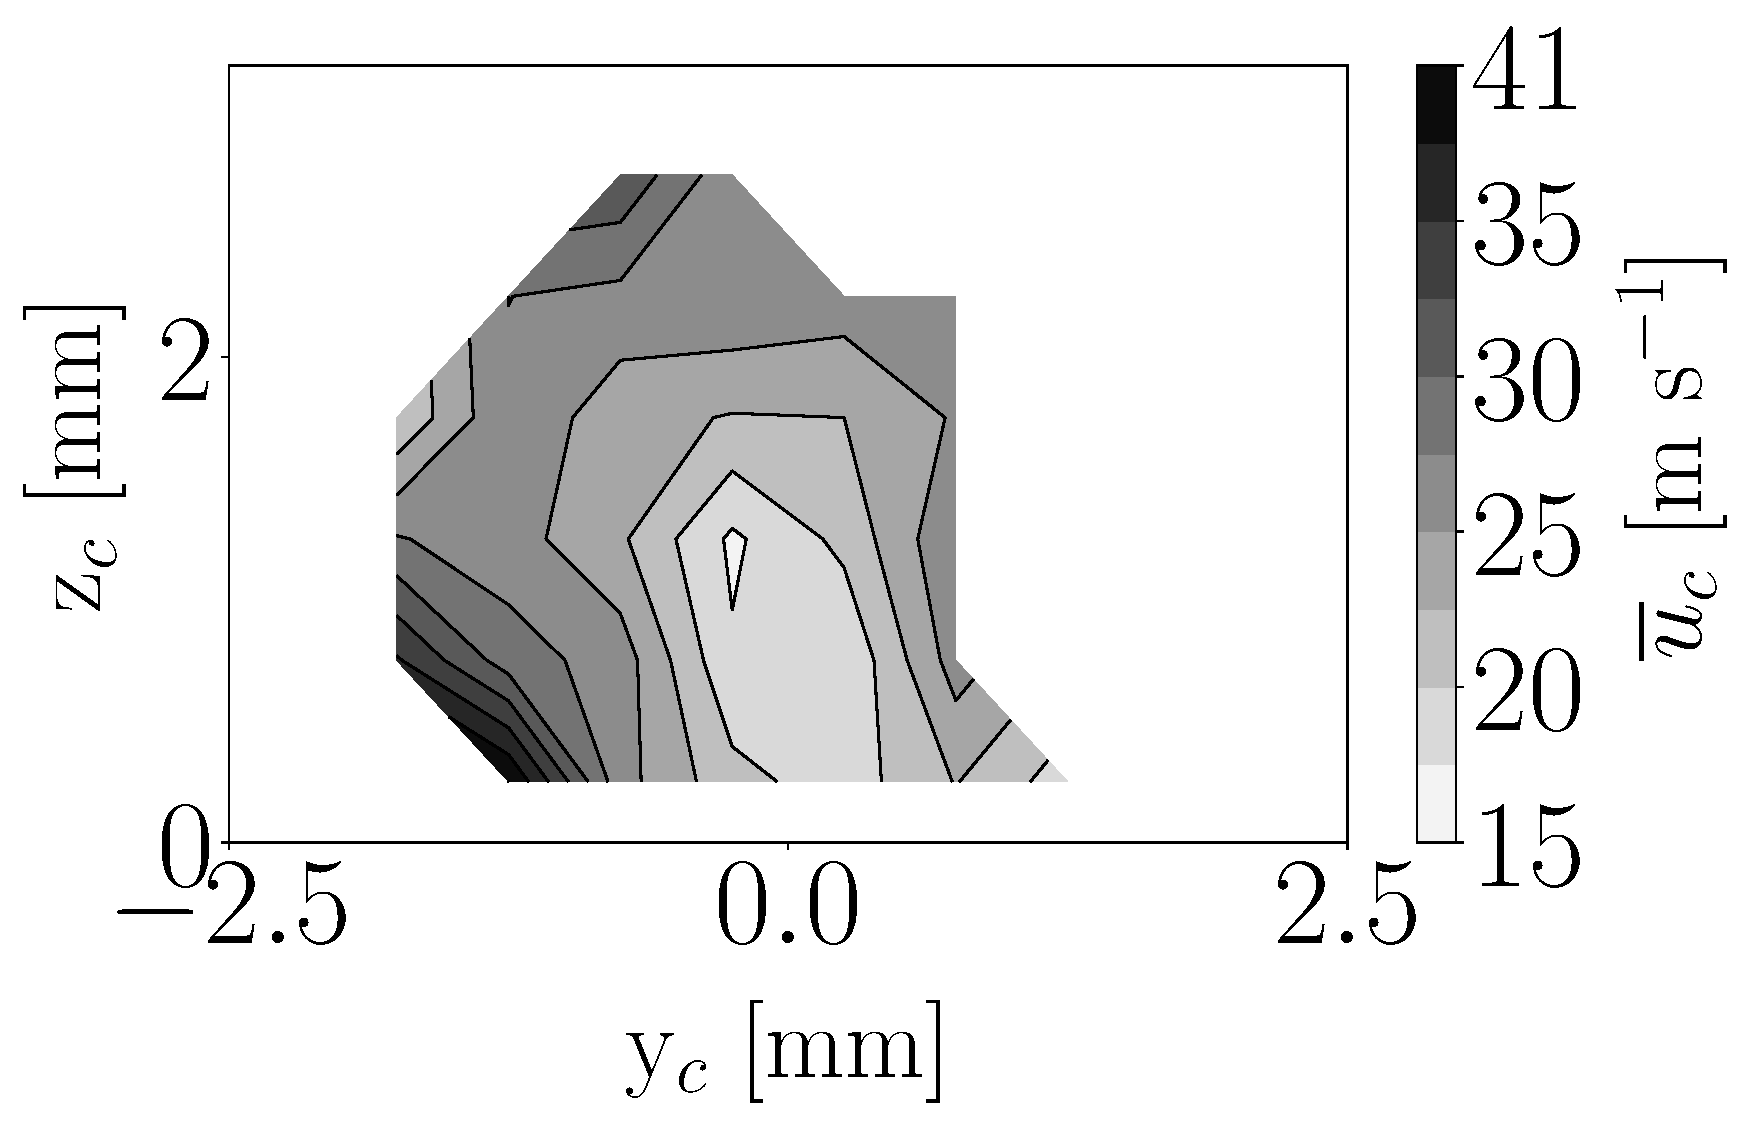
\includegraphics[scale=\scaleSLIBIMER]{./part3_applications/figures_ch8_resolved/injectors_SLI/dx15_xD05p00_ux_mean_map}
   %\caption{Case UG100\_DX20: crossflow planes}
   %\label{} 
\end{subfigure}
   \hspace{0.17in}
\begin{subfigure}[b]{0.3\textwidth}
	\centering
   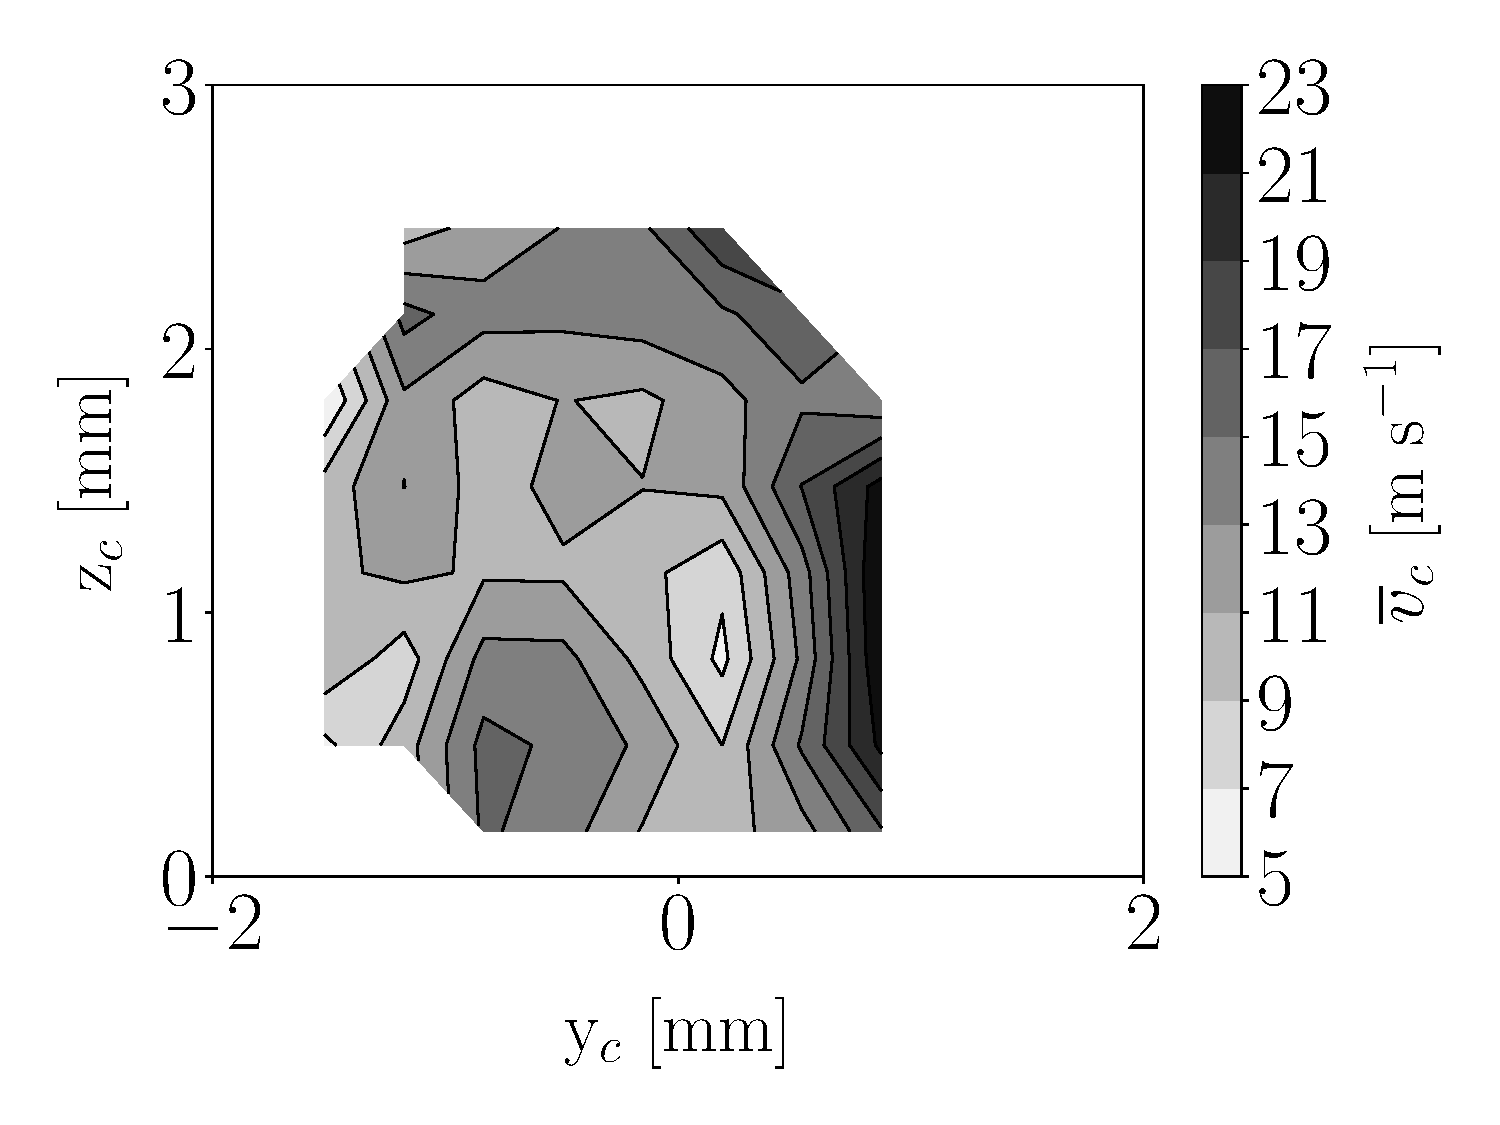
\includegraphics[scale=\scaleSLIBIMER]{./part3_applications/figures_ch8_resolved/injectors_SLI/dx15_xD05p00_uy_mean_map}
   %\caption{Case UG100\_DX20: filming planes}
   %\label{}
\end{subfigure}
   \hspace{0.17in}
\begin{subfigure}[b]{0.3\textwidth}
	\centering
   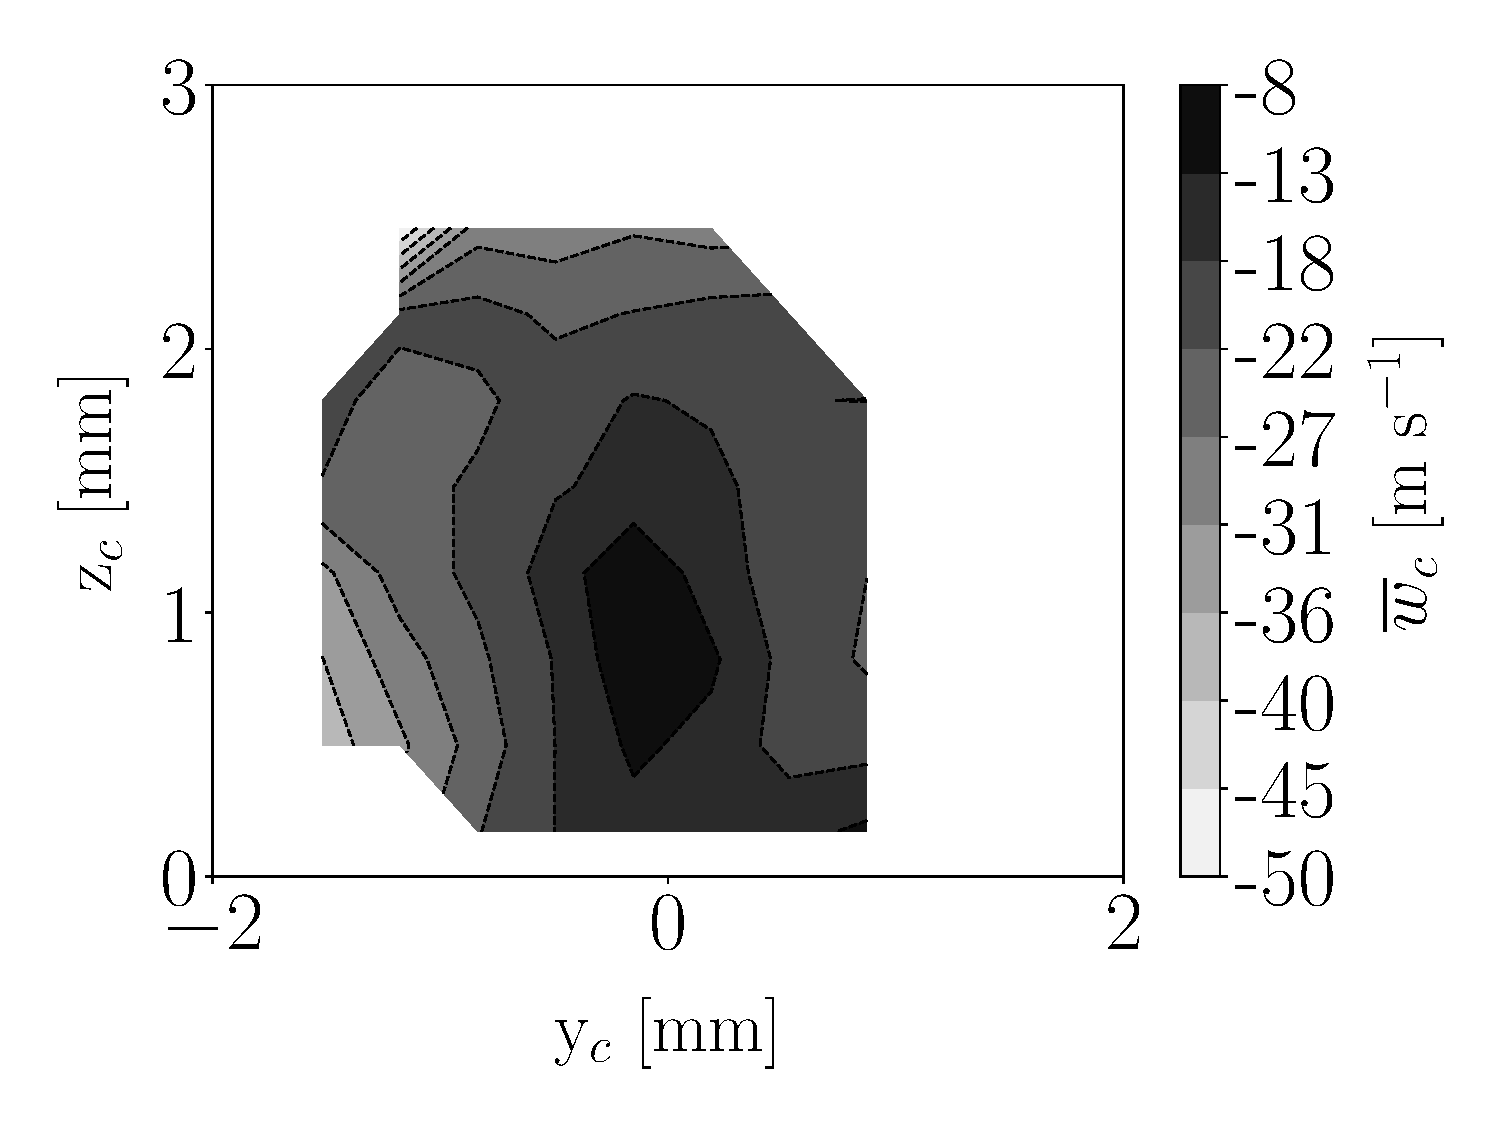
\includegraphics[scale=\scaleSLIBIMER]{./part3_applications/figures_ch8_resolved/injectors_SLI/dx15_xD05p00_uz_mean_map}
   %\caption{Case UG100\_DX10: crossflow planes}
   %\label{} 
\end{subfigure}
\caption{Spray states at $x_c$ = 1.5 mm for case DX15}
%\caption{Spray states at $x/d_\mathrm{inj}$ = 5 for case DX15}
\label{fig:injectors_sli_BIMER_DX15_xD05}
\end{figure}

%%%%%%%%%%%%%%%% DX15, xD = 6.67


\begin{figure}[h!]
\centering
\begin{subfigure}[b]{0.3\textwidth}
	\centering
   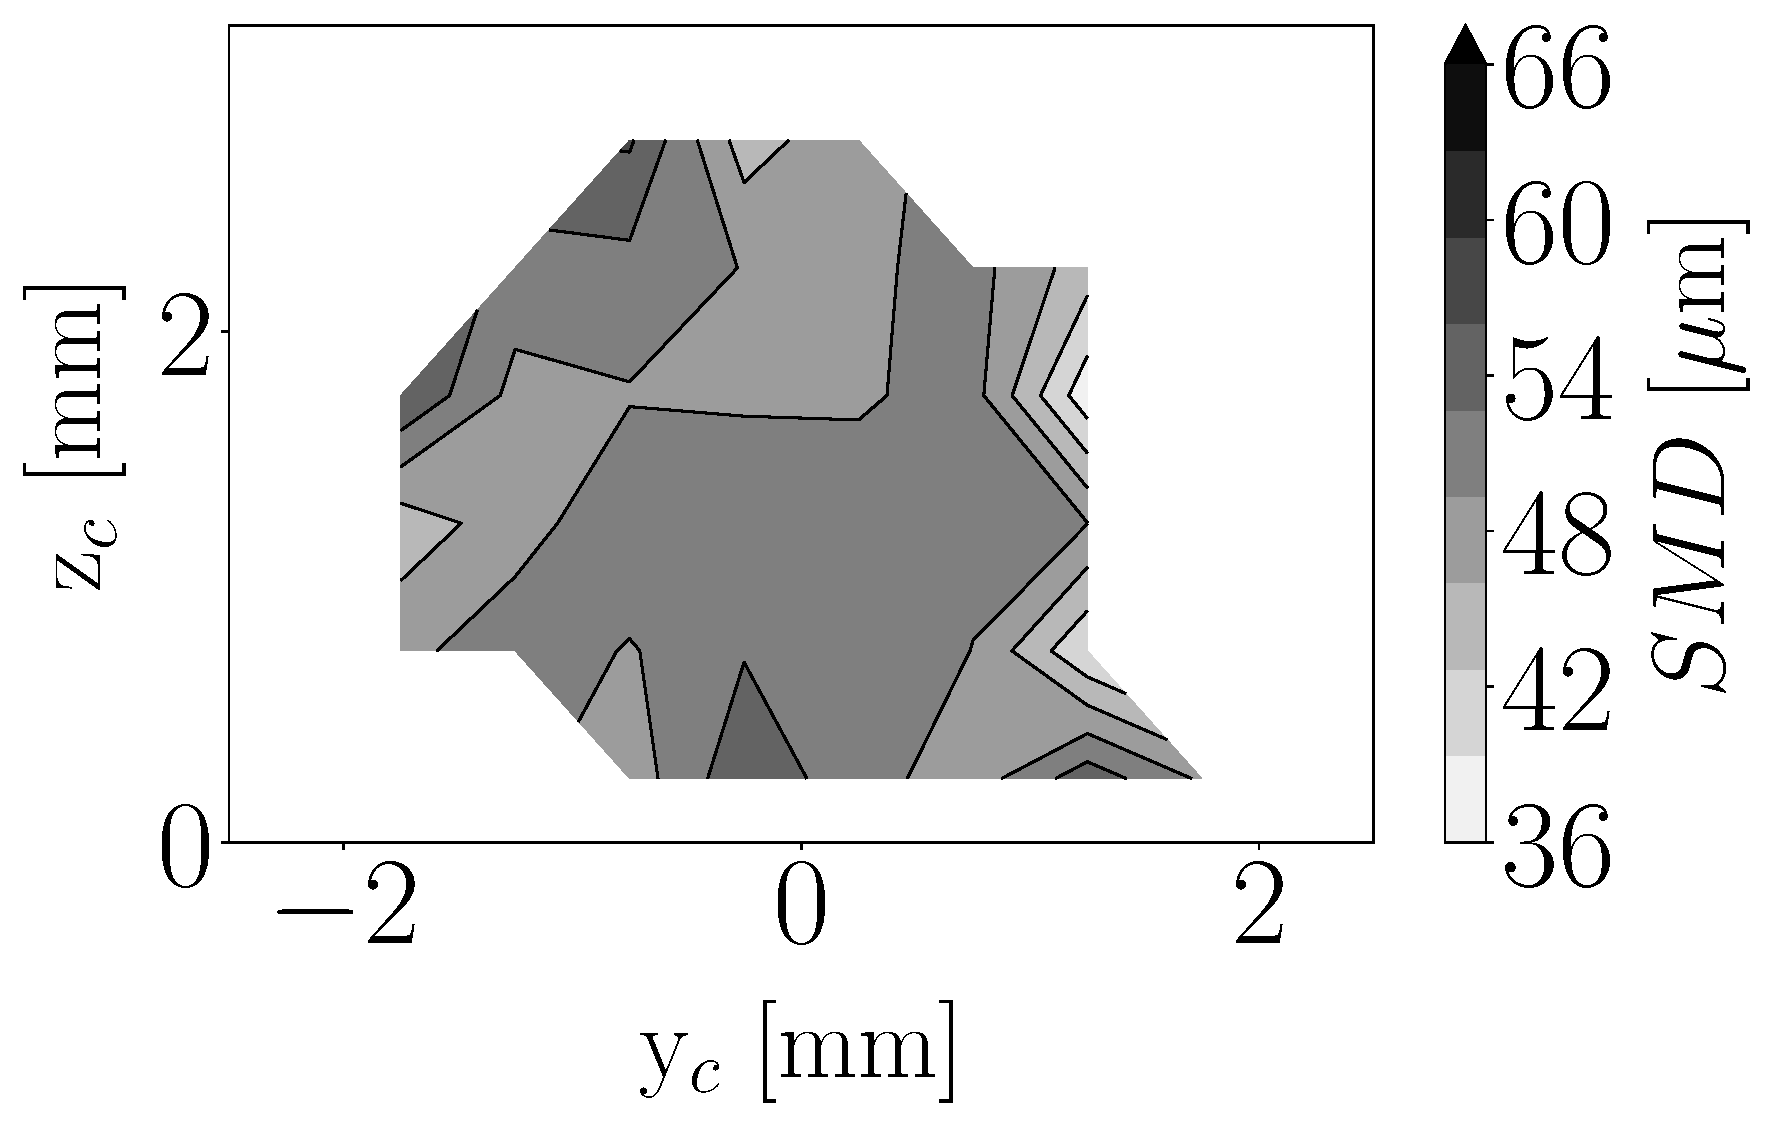
\includegraphics[scale=\scaleSLIBIMER]{./part3_applications/figures_ch8_resolved/injectors_SLI/dx15_xD06p67_SMD_map}
   %\caption{Case UG100\_DX20: crossflow planes}
   %\label{} 
\end{subfigure}
   \hspace{0.17in}
\begin{subfigure}[b]{0.3\textwidth}
	\centering
   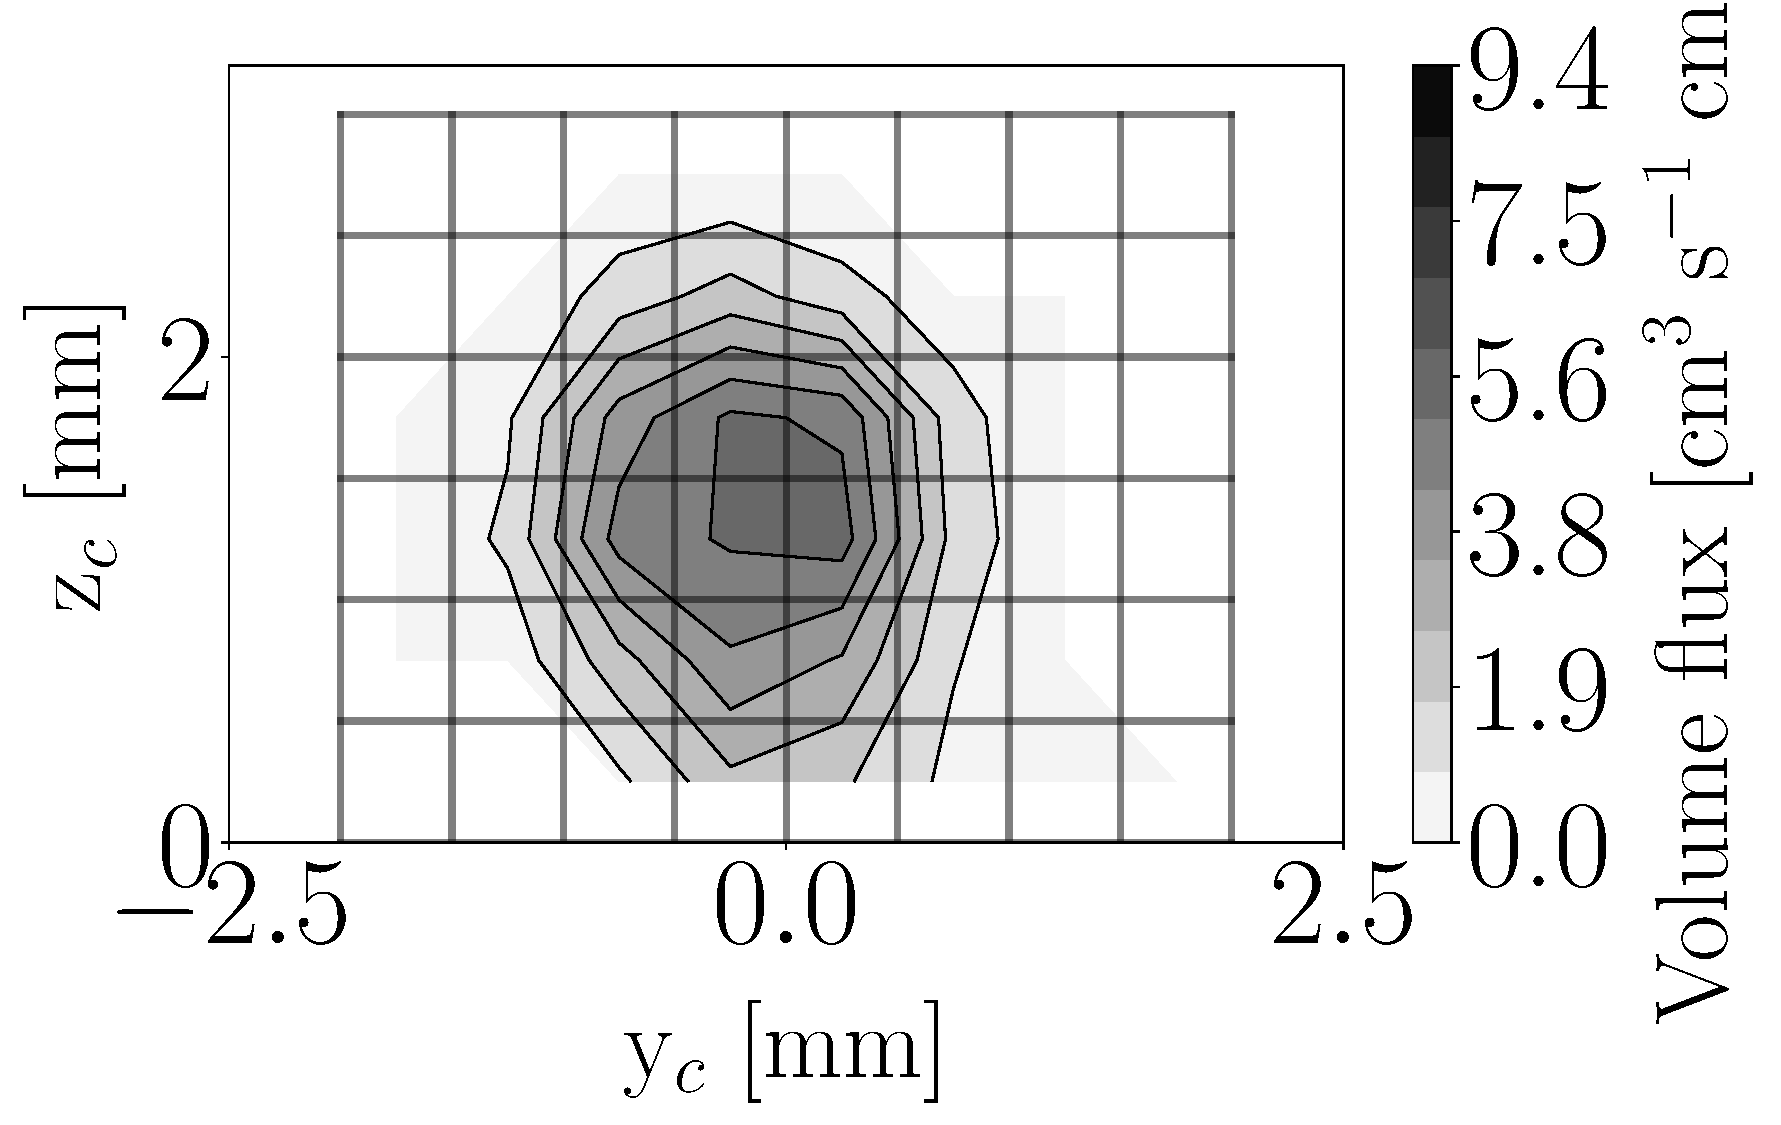
\includegraphics[scale=\scaleSLIBIMER]{./part3_applications/figures_ch8_resolved/injectors_SLI/dx15_xD06p67_volume_flux_map}
   %\caption{Case UG100\_DX20: filming planes}
   %\label{}
\end{subfigure}
   \hspace{0.17in}
\begin{subfigure}[b]{0.3\textwidth}
	\centering
   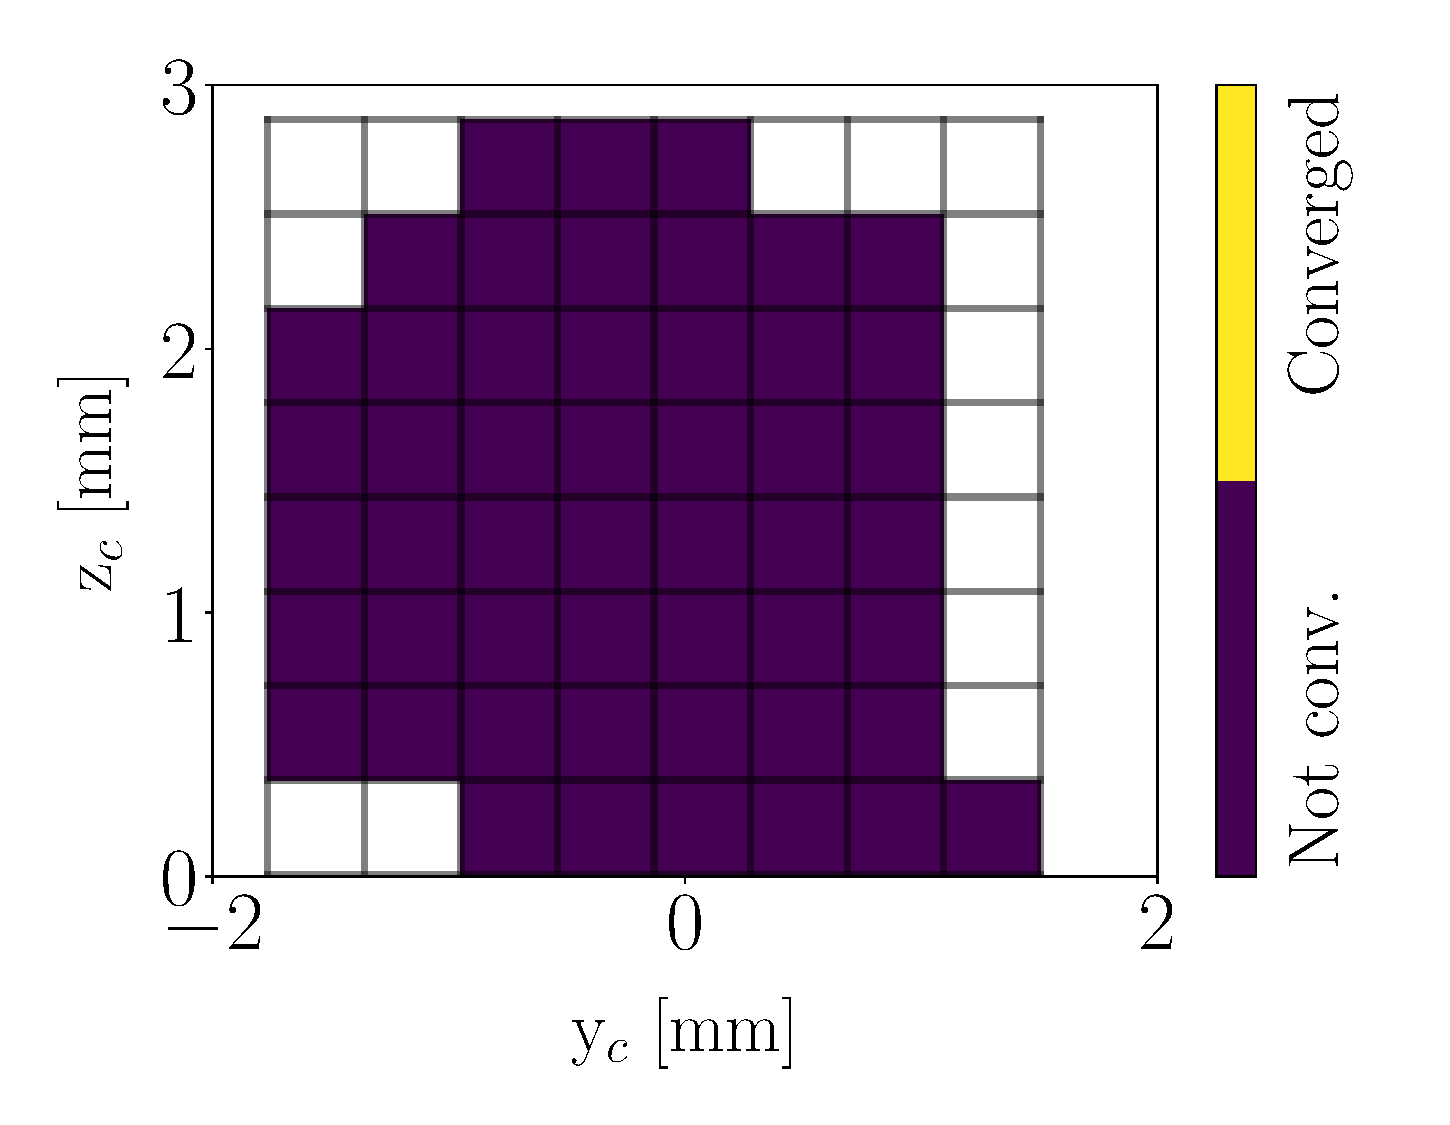
\includegraphics[scale=\scaleSLIBIMER]{./part3_applications/figures_ch8_resolved/injectors_SLI/dx15_xD06p67_convergence_map}
   %\caption{Case UG100\_DX10: crossflow planes}
   %\label{} 
\end{subfigure}

\vskip\baselineskip

\begin{subfigure}[b]{0.3\textwidth}
	\centering
   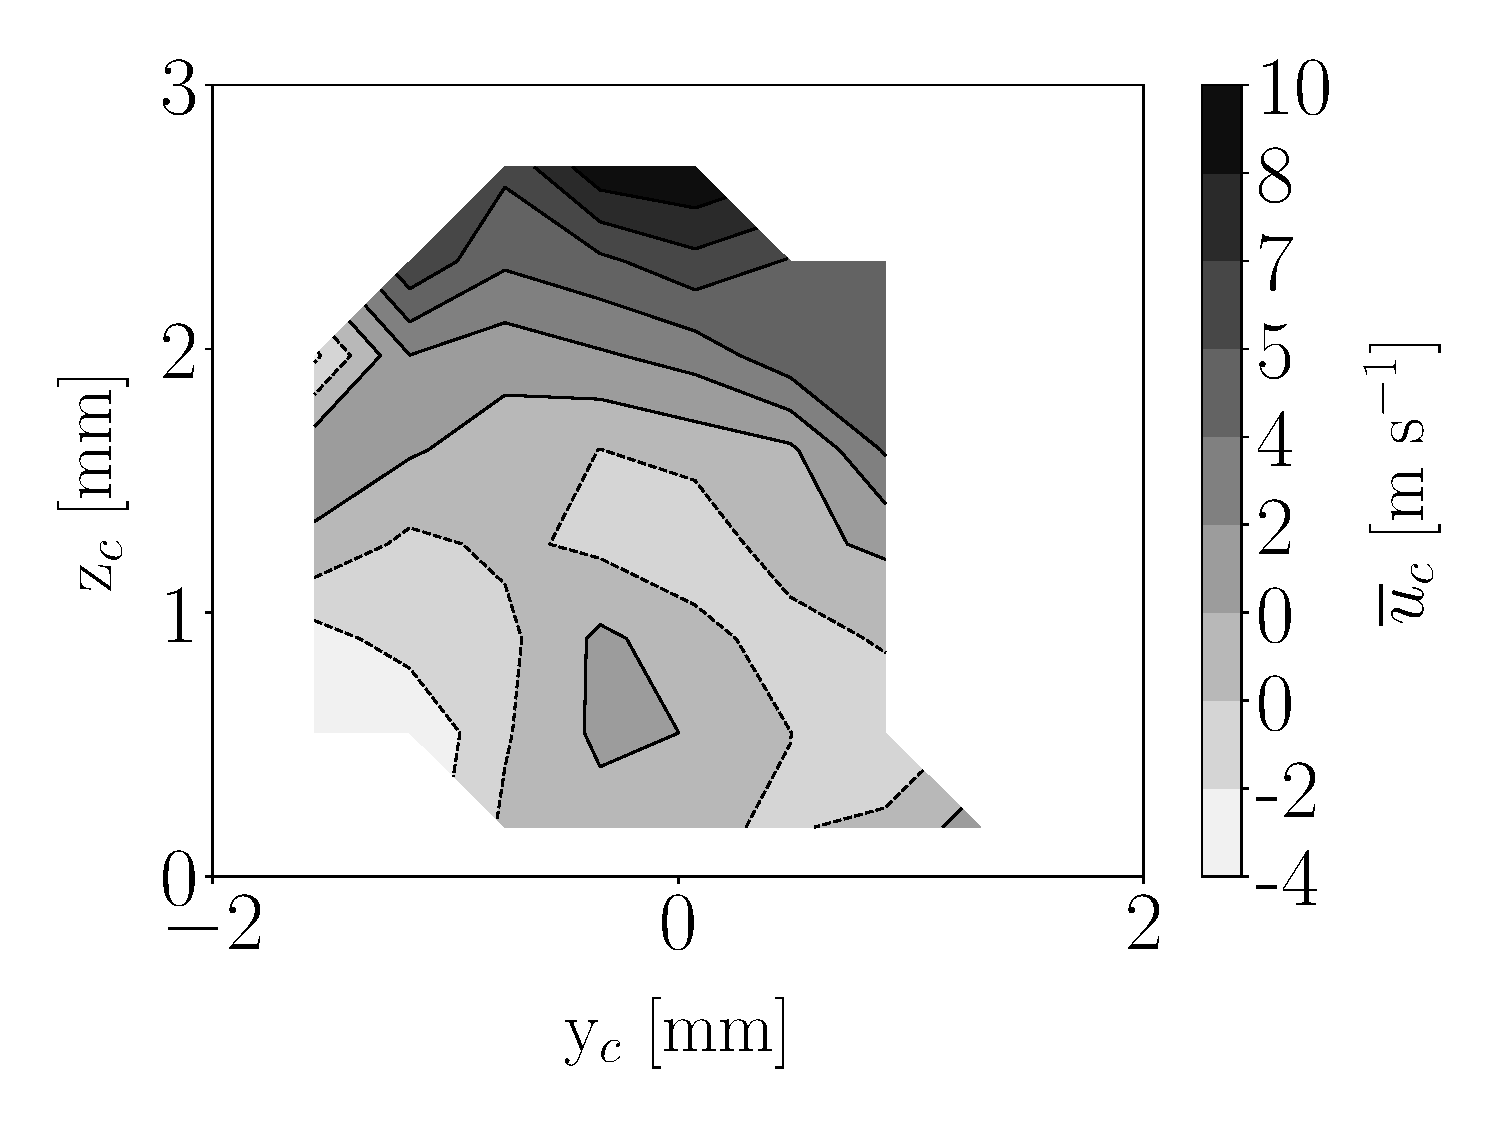
\includegraphics[scale=\scaleSLIBIMER]{./part3_applications/figures_ch8_resolved/injectors_SLI/dx15_xD06p67_ux_mean_map}
   %\caption{Case UG100\_DX20: crossflow planes}
   %\label{} 
\end{subfigure}
   \hspace{0.17in}
\begin{subfigure}[b]{0.3\textwidth}
	\centering
   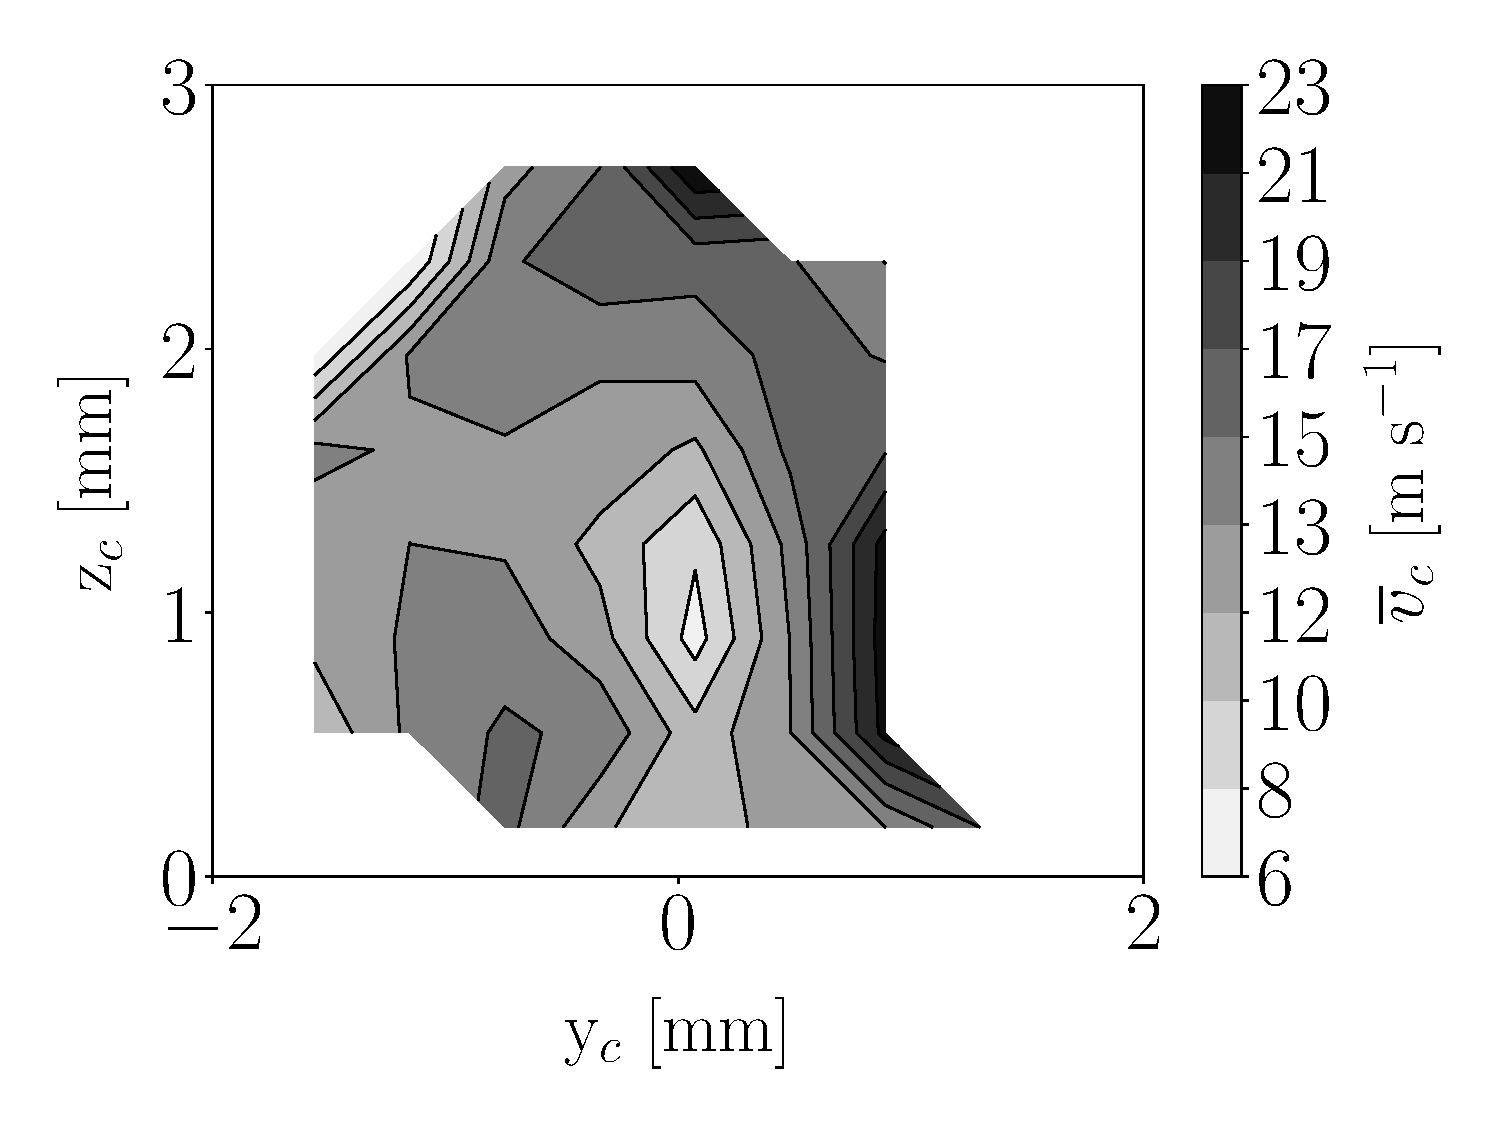
\includegraphics[scale=\scaleSLIBIMER]{./part3_applications/figures_ch8_resolved/injectors_SLI/dx15_xD06p67_uy_mean_map}
   %\caption{Case UG100\_DX20: filming planes}
   %\label{}
\end{subfigure}
   \hspace{0.17in}
\begin{subfigure}[b]{0.3\textwidth}
	\centering
   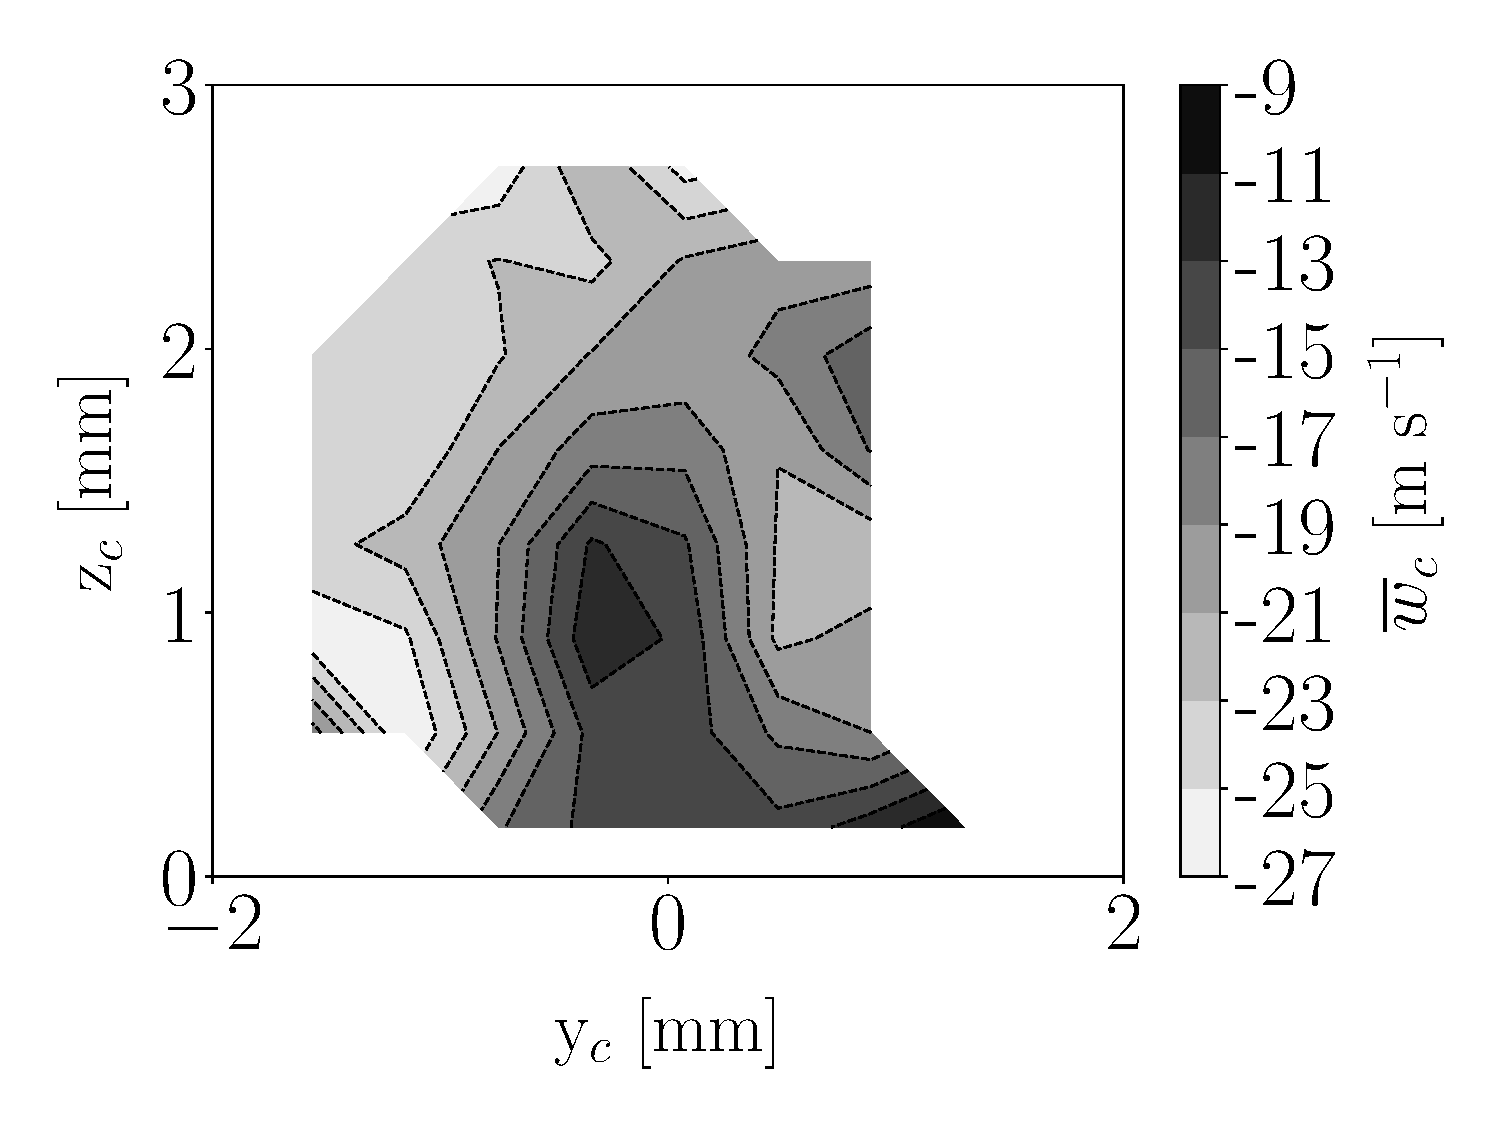
\includegraphics[scale=\scaleSLIBIMER]{./part3_applications/figures_ch8_resolved/injectors_SLI/dx15_xD06p67_uz_mean_map}
   %\caption{Case UG100\_DX10: crossflow planes}
   %\label{} 
\end{subfigure}
\caption{Spray states at $x_c$ = 2 mm for case DX15}
%\caption{Spray states at $x/d_\mathrm{inj}$ = 6.67 for case DX15}
\label{fig:injectors_sli_BIMER_DX15_xD06p67}
\end{figure}
